% !arara: pdflatex
% !arara: biber
% arara: pdflatex
% arara: pdflatex
% --------------------------------------------------------------------------
% the CHEMMACROS package
%
%   macros and commands for chemists
%
% --------------------------------------------------------------------------
% Clemens Niederberger
% --------------------------------------------------------------------------
% https://github.com/cgnieder/chemmacros/
% contact@mychemistry.eu
% --------------------------------------------------------------------------
% If you have any ideas, questions, suggestions or bugs to report, please
% feel free to contact me.
% --------------------------------------------------------------------------
% Copyright 2011-2014 Clemens Niederberger
%
% This work may be distributed and/or modified under the
% conditions of the LaTeX Project Public License, either version 1.3
% of this license or (at your option) any later version.
% The latest version of this license is in
%   http://www.latex-project.org/lppl.txt
% and version 1.3 or later is part of all distributions of LaTeX
% version 2005/12/01 or later.
%
% This work has the LPPL maintenance status `maintained'.
%
% The Current Maintainer of this work is Clemens Niederberger.
% --------------------------------------------------------------------------
\documentclass[load-preamble+]{cnltx-doc}
\usepackage[utf8]{inputenc}
\usepackage[greek=newtx]{chemmacros}
\setcnltx{
  package  = {chemmacros},
  info     = {macros and commands for chemists},
  url      = https://github.com/cgnieder/chemmacros/ ,
  authors  = Clemens Niederberger ,
  email    = contact@mychemistry.eu ,
  abstract = {%
    \centering
    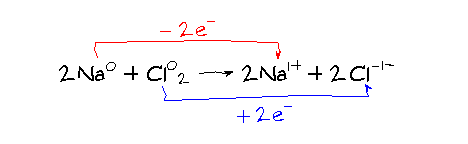
\includegraphics{chemmacros-logo.pdf}
    \par
  } ,
  add-cmds = {
     abinitio, activatechemgreekmapping, AddRxnDesc, anti, aq, aqi,
     ba, bond, bridge,
    cd, ch, changechemgreeksymbol, charrow, chcpd, chemabove, chemalpha,
      chembeta, chemgamma, chemdelta, chemDelta, chemformula@bondlength,
      chemomega, chemphi, chemPhi, chemsetup, chlewis, chname , cip, cis, ch,
      CNMR,
    data, DeclareChemArrow, DeclareChemBond, DeclareChemBondAlias,
      declarechemgreekmapping, DeclareChemIUPAC, DeclareChemLatin,
      DeclareChemNMR, DeclareChemParticle, DeclareChemPhase,
      DeclareChemReaction, DeclareChemState, delm, delp, Delta, Dfi,
    el, ElPot, endo, Enthalpy, enthalpy, Entropy,
    fmch, fpch, fscrm, fscrp,
    gas, ghs, ghslistall, ghspic, Gibbs, gram,
    hapto, HNMR, Helmholtz, hydrogen,
    insitu, invacuo, iupac,
    Ka, Kb, Kw,
    Lfi, listofreactions, lqd,
    mch, mega, meta, mhName,
    NewChemArrow, NewChemBond, NewChemBondAlias,
      newchemgreekmapping, NewChemIUPAC, NewChemLatin,
      NewChemNMR, NewChemParticle, NewChemPhase,
      NewChemReaction, NewChemState,
      newman, nitrogen, NMR, Nu, Nuc,
    orbital, ortho, ox, OX, oxygen,
    para, pch, per, pH, phase, phosphorus, photon, pKa, pKb, pOH, pos,
      positron, Pot, prt,
    Rad, redox, RenewChemArrow, RenewChemBond, renewchemgreekmapping,
      RenewChemIUPAC, RenewChemLatin, RenewChemNMR, RenewChemParticle,
      RenewChemPhase, RenewChemState,
    Sf, scrm, scrp, second, selectchemgreekmapping, setchemformula,
      ShowChemArrow, ShowChemBond, sld, Sod, State, sulfur,
    trans,
    val
  } ,
  add-silent-cmds = {
    addplot,
    bottomrule,
    cancel, cdot, ce, cee, celsius, centering, chemfig, chemname, clap,
      cnsetup, color, cstack, cstsetup,
    DeclareInstance, DeclareSIUnit, definecolor, draw,
    electronvolt,
    footnotesize,
    glqq, grqq,
    hertz, hspace,
    includegraphics, intertext, IUPAC,
    joule,
    kilo,
    latin, lewis, Lewis, liquid, ltn,
    metre, midrule, milli, mmHg, mole,
    nano, nicefrac, num, numrange,
    ominus, oplus,
    percent, pgfarrowsdeclarealias, pgfarrowsrenewalias,
    renewtagform, rightarrow,
    sample, scriptscriptstyle, setatomsep, setbondoffset, sfrac, shorthandoff,
      si, SI, sisetup, square, subsection,
    textcolor, textendash, textsuperscript, tiny, toprule,
    upbeta, upeta, upgamma, usetikzlibrary,
    volt, vphantom, vspave,
    xspace,
    z@, z@skip
  }
}

\usepackage{chemfig,booktabs,cancel,varioref,csquotes}

\expandafter\def\csname libertine@figurestyle\endcsname{LF}
\usepackage[libertine]{newtxmath}
\expandafter\def\csname libertine@figurestyle\endcsname{OsF}

\usepackage[biblatex]{embrac}
\ChangeEmph{[}[,.02em]{]}[.055em,-.08em]
\ChangeEmph{(}[-.01em,.04em]{)}[.04em,-.05em]

\usepackage[accsupp]{acro}
\acsetup{
  long-format  = \scshape ,
  short-format = \scshape
}
\DeclareAcronym{ghs}{
  short     = ghs ,
  long      = Globally Harmonized System of Classification and Labelling of
    Chemicals ,
  pdfstring = GHS ,
  accsupp   = GHS
}
\DeclareAcronym{eu}{
  short     = EU ,
  long      = European Union ,
  pdfstring = EU ,
  accsupp   = EU
}
\DeclareAcronym{iupac}{
  short     = iupac ,
  long      = International Union of Pure and Applied Chemistry ,
  pdfstring = IUPAC ,
  accsupp   = IUPAC
}
\DeclareAcronym{UN}{
  short     = un ,
  long      = United Nations ,
  pdfstring = UN ,
  accsupp   = UN
}
\DeclareAcronym{dvi}{
  short     = dvi ,
  long      = device independent file format ,
  pdfstring = DVI ,
  accsupp   = DVO
}
\DeclareAcronym{pdf}{
  short     = pdf ,
  long      = portable document file ,
  pdfstring = PDF ,
  accsupp   = PDF
}
\DeclareAcronym{id}{
  short     = id ,
  long      = identification string ,
  pdfstring = ID ,
  accsupp   = ID
}

\chemsetup{
  option/synchronize ,
  chemformula/format = \libertineLF
}

\sisetup{
  detect-mode=false,
  mode=text,
  text-rm=\libertineLF
}

\usepackage{filecontents}

\defbibheading{bibliography}{\addsec{References}}
\addbibresource{\jobname.bib}
\begin{filecontents*}{\jobname.bib}
@book{iupac:greenbook,
  author    = {E. Richard Cohan and Tomislav Cvita\v{s} and Jeremy G. Frey and
    Bertil Holmstr\"om and Kozo Kuchitsu and Roberto Marquardt and Ian Mills and
    Franco Pavese and Martin Quack and J\"urgen Stohner and Herbert L. Strauss and
    Michio Takami and Anders J Thor} ,
  title     = {``Quantities, Symbols and Units in Physical Chemistry'', \acs{iupac}
    Green Book} ,
  sorttitle = {Quantities, Symbols and Units in Physical Chemistry} ,
  indexsorttitle = {Quantities, Symbols and Units in Physical Chemistry} ,
  edition   = {3rd Edition. 2nd Printing} ,
  year      = {2008} ,
  publisher = {\acs{iupac} \&\ RSC Publishing, Cambridge}
}
@book{iupac:redbook,
  author    = {Neil G. Connelly and Ture Damhus and Richard M. Hartshorn and
    Alan T. Hutton} ,
  title     = {``Nomenclature of Inorganic Chemistry'', \acs{iupac} Red Book} ,
  sorttitle = {Nomenclature of Inorganic Chemistry} ,
  indexsorttitle = {Nomenclature of Inorganic Chemistry} ,
  year      = {2005} ,
  publisher = { \acs{iupac} \&\ RSC Publishing, Cambridge} ,
  isbn      = {0-85404-438-8}
}
@book{iupac:bluebook,
  author    = {R. Panico and W. H. Powell and J-C. Richer},
  title     = {``Nomenclature of Organic Chemistry, Sections A, B, C, D, E, F,
    and H'', \acs{iupac} Blue Book},
  sorttitle = {Nomenclature of Organic Chemistry} ,
  indexsorttitle = {Nomenclature of Organic Chemistry} ,
  edition   = {\mkbibacro{draft}},
  date      = {2004-10-07},
  url       =
  {http://old.iupac.org/reports/provisional/abstract04/BB-prs310305/CompleteDraft.pdf},
  urldate   = {2013-07-07}
}
@misc{eu:ghsystem_regulation,
  author   = {{The European Parliament and The Council of the European Union}},
  sortname = {European Parliament and The Council of the European Union} ,
  title    = {Regulation (EC) No 1272/2008 of the European Parliament and of
    the Council} ,
  subtitle = {on classification, labelling and packaging of substances and
    mixtures, amending and repealing Directives 67/548/EEC and 1999/45/EC, and
    amending Regulation (EC) No 1907/2006} ,
  journal  = {Official Journal of the European Union} ,
  date     = {2008-12-16}
}
@online{unece:ghsystem_implementation,
  author   = {{United Nations Economic Commission for Europe}} ,
  title    = {GHS Implementation} ,
  url      =
    {http://www.unece.org/trans/danger/publi/ghs/implementation_e.html} ,
  urldate  = {2012-03-20} ,
  date     = {2012-03-20}
}
\end{filecontents*}

\DeclareInstance{xfrac}{chemformula-text-frac}{text}
  {
    scale-factor        = 1 ,
    denominator-bot-sep = -.2ex ,
    denominator-format  = \scriptsize #1 ,
    numerator-top-sep   = -.2ex ,
    numerator-format    = \scriptsize #1 ,
    slash-right-kern    = .05em ,
    slash-left-kern     = .05em
  }

\usetikzlibrary{calc,positioning,decorations.pathmorphing,patterns}

% \newpackagename\chemmacros{chemmacros}
\newpackagename\chemformula{chemformula}
\newpackagename\ghsystem{ghsystem}
\newpackagename\chemgreek{chemgreek}

\renewcommand*\AmS{\hologo{AmS}}
\newcommand*\TikZ{Ti\textit{k}Z}
\newcommand*\tablehead[1]{\textrm{\bfseries#1}}

\NewChemPhase{\aqi}{aq,$\infty$}% aqueous solution at infinite dilution
\NewChemPhase{\cd}{cd}% condensed phase
\NewChemPhase{\lc}{lc}% liquid crystal

\newname\hensel{Martin Hensel}
\newname\pedersen{Bj\o rn Pedersen}

\BeforeBeginEnvironment{example}{\vspace{\baselineskip}}
\AfterEndEnvironment{example}{\vspace{\baselineskip}}
\BeforeBeginEnvironment{sourcecode}{\vspace{\baselineskip}}
\AfterEndEnvironment{sourcecode}{\vspace{\baselineskip}}

\begin{document}

\part{Preliminaries}
\section{Licence, Requirements and \textsc{README}}
\license

The \chemmacros\ package needs the bundles \bnd{l3kernel}~\cite{bnd:l3kernel}
and \bnd{l3packages}~\cite{bnd:l3packages}.  It also needs the packages
\needpackage{siunitx}~\cite{pkg:siunitx},
\needpackage{mathtools}~\cite{pkg:mathtools}, \needpackage{bm}~\cite{pkg:bm},
\needpackage{nicefrac}~\cite{pkg:nicefrac} and
\needpackage{environ}~\cite{pkg:environ} as well as
\pkg{tikz}\footnote{\CTANurl[graphics]{pgf}}~\cite{pkg:pgf} and the \TikZ\
libraries \code{calc} and \code{arrows}.  Language support is done with the
help of the \needpackage{translations}~\cite{pkg:translations}.  The
\chemmacros\ package also loads the packages
\pkg{chemformula}~\cite{pkg:chemformula} and
\pkg{chemgreek}~\cite{pkg:chemgreek}.

The package option \option{xspace} also loads the package
\pkg{xspace}~\cite{pkg:xspace}.

The package option \option{ghsystem} also loads the package
\pkg{ghsystem}~\cite{pkg:ghsystem}.


\section{Motivation and Background}
\chemmacros\ started some years ago as a growing list of custom macros that I
frequently used.  I cannot completely recall when and why I decided to release
them as a package.  Well -- here we go and you might find it useful, too, I
hope.

Both the macros and their functionality have changed over time and quite a lot
have been added.  Many things have been unified and what's probably most
important: many possibilities to customize have been added, too.

Probably every chemist using \LaTeXe\ is aware of the great \pkg{mhchem}
package by \hensel.  There have always been some difficulties intertwining it
with \chemmacros, though.  Also, some other minor points in \pkg{mhchem}
always bothered me, but they hardly seemed enough for a new package.  They
weren't even enough for a feature request to the \pkg{mhchem} author.  The
challenge and the fun of creating a new package and the wish for a highly
customizable alternative led to \chemformula\ after all.  \chemformula{} used
to part of \chemmacros{} for quite a while but now is an independent package.

As a chemist you are probably aware of the fact that the \acl{UN} have
developed the \ac{ghs} as a global replacement for the various different
systems in different countries.  While it has not been implemented by all
countries yet~\cite{unece:ghsystem_implementation}, it is only a matter of
time.

The package \ghsystem\ enables you to typeset all the hazard and precautionary
statements and pictograms in a very easy way.  The statements are taken from
\acs{eu} regulation 1272/2008~\cite{eu:ghsystem_regulation}.  \ghsystem{} used
to be a part of \chemmacros{} for quite a while but now is an independent
package.

There are four points I hope I have achieved with this package:
\begin{itemize}
  \item intuitive usage as far as the syntax of the commands is concerned
  \item the commands shall not only make typesetting easier and faster but also
    the document source more readable with respect to semantics
    (\code{\cs{ortho}-dichlorobenzene} is easier to read and understand than
    \code{\cs*{textit}\Marg{o}-dichlorobenzene})
  \item as much customizability as I could think of so every user can adapt the
    commands to his or her own wishes
  \item default settings compliant with the recommendations of the \acf{iupac}.
\end{itemize}
Especially the last point needed some pushing from users to get things right
in many places.  If you find anything not compliant with \ac{iupac}
recommendations\footnote{This does not concern the \cs{ox} command. The
  \ac{iupac} version is \cs{ox}\sarg.} I would welcome an email very much!

\section{News}
\subsection{Version~4.0}
With version~4.0 some changes have been made:
\begin{itemize}
  \item first of all the packages \chemformula\ and \ghsystem\ do not load
    \chemmacros\ any more which means they can be used independently.
  \item the option \option{bpchem} has been dropped.
  \item the commands \cs{mch} and \cs{pch} now match \chemformula's
    charges.
  \item the option \option{method} has been dropped.
  \item the option \option{append} has deprecated.
  \item the option \option{greek} has been extended to support other uppercase
    greek letters, for example those provided by \pkg{kpfonts}.  This is
    handled internally by the new package in the family: \chemgreek.  This
    package is not really a package for usage at a user-level but could in
    principle be used to extend the \option{greek} option.
  \item language support is now done with the help of the \pkg{translations}.
    This means that with version~4.0  the document language is recognized
    automatically.
  \item the status of the commands \cs{Lfi} and \cs{Dfi} has been changed
    from \emph{deprecated} to \emph{dropped}.
  \item various other changes like bug fixes and improvements on the
    typographical appearance of \chemformula's inline formulae with \cs{ch}.
\end{itemize}

\subsection{Version~4.2}

\begin{itemize}
  \item Changed particles with electron pairs such as \cs{ba} to use
    \chemformula's new macro \cs{chlewis} for the Lewis electrons.
  \item Changed the implicit \cs*{Delta} in the thermodynamic state variables
    into \cs*{ChemDelta} to ensure that an upright symbol is used.
  \item Change in the syntax of \cs{DeclareChemState} and
    \cs{RenewChemState}.  The old syntax is still supported but discouraged.
\end{itemize}

\subsection{Version 4.3}
\begin{itemize}
  \item All one-letter \acs{iupac} macros have been exchanged in favour of
    more meaningful macro names.  The one-letter commands still exist for
    backward compatibility (and to some users no doubt also for convenience).
    They are no longer recommended though.  One-letter commands seldomly have
    meaningful names and  often they've also been defined by other packages.
    This means they make collaboration more difficult than it needs to be and
    are a source for package conflicts.  \chemmacros\ used to solved the
    latter problem by only providing them inside the argument of
    \cs{iupac}\label{desc:one-letter-commands}.  The one exception
    \chemmacros\ makes is the command \cs{p} (for things like \pH) which is
    and will remain an official command.
  \item The environment \env{experimental} has got a number of new options,
    see section~\ref{sec:experimental-customization}.
  \item The commands \cs*{DeclareChem\meta{...}} now don't give an error any
    more if the command already exists.  This is more consistent with \LaTeX's
    \cs*{DeclareRobustCommand}.  For all those commands a version
    \cs*{NewChem\meta{...}} is introduced that \emph{does} give an error if
    the new command is already defined.
  \item The package option \option{strict} has been deprecated.
  \item The package option \option{cmversion} has been deprecated.
  \item The command \cs{mhName} has been dropped.
\end{itemize}

\subsection{Version 4.4}
\begin{itemize}
  \item New \module{nmr} option \option{atom-number-cs}.
  \item New \module{nmr} option \option{coupling-pos-cs}.
\end{itemize}

\subsection{Version 4.5}
\begin{itemize}
  \item New \module{acid-base} option \option{subscript}.
  \item Dutch translations.
\end{itemize}

\subsection{Version 4.6}
\begin{itemize}
  \item The packages \chemformula, \chemgreek{} and \ghsystem{} are no longer
    distributed as a part of \chemmacros{} but as packages of their own.
  \item Inside \cs{iupac} the characters \code{\textbar} and
    \code{\textasciicircum} are active.  The corresponding commands
    \cs{\textbar} and \cs{\textasciicircum} are deprecated now and will be
    dropped eventually.
\end{itemize}

\section{Package Options}\label{sec:options}
\chemmacros\ has several package options. They all are used as key/value pairs
like
\begin{sourcecode}
  \usepackage[option1 = <value1>, option2 = <value2>]{chemmacros}
\end{sourcecode}
Some also can be used without value
(\verbcode+\usepackage[option1]{chemmacros}+), which means that the
\default{underlined} value is used.

\begin{options}
  % circled
  \keychoice{circled}{formal,\default{all},none}\Module{option}\Default{formal}
    \chemmacros\ uses two different kinds of charges which indicate the usage
    of real ($+/-$) and formal (\fplus/\fminus) charges.  The option
    \code{formal} distinguishes between them, option \code{none} displays them
    all without circle, option \code{all} circles all.
  % circletype
  \keychoice{circletype}{\default{chem},math}\Module{option}\Default{chem}
    This option switches between two kinds of circled charge symbols:
    \cs{fplus} \fplus\ and \verbcode+$\oplus$+ $\oplus$.
  % ghsystem
  \keybool{ghsystem}\Module{option}\Default{false}
    \keyis{ghsystem}{false} disables the automatic loading of the \ghsystem\
    package.
  % greek
  \keychoice{greek}{\default{auto},upgreek,textgreek,mathdesign,kpfonts,newtx,%
      fourier,textalpha}\Module{option}{}% empty group pushes default value to
                                         % next line
    \Default{auto}
    This option determines how the letters \cs{chemalpha} and friends are
    typeset.  See pages~\pageref{desc:greek} and~\pageref{par:greek_letters}
    for more information.  Please note that this option \emph{does not load
      either \pkg{upgreek}, \pkg{kpfonts} or any other package!}  It only
    determines which one to choose if available.  The option \code{auto} will
    detect if any of the packages needed for one of the options has been
    loaded and use it if available.  If more than one of the packages has been
    loaded the option will choose the one listed first in the above choice
    list.  If you explicitly choose an option other than \code{auto} or
    \code{math} you also have to load the corresponding package.  \emph{This
      option can only be chosen in the preamble}.
  % iupac
  \keychoice{iupac}{auto,restricted,strict}\Module{option}\Default{auto}
    Take care of how \ac{iupac} naming commands are defined, see
    page~\pageref{desc:iupac}.
  % language
  \keychoice{language}{american,british,english,french,german,italian,ngerman}%
    \Module{option}\Default
    Load the language used by \chemmacros.  \emph{This option can only be
      chosen in the preamble}.
  % Nu
  \keychoice{Nu}{\default{chemmacros},mathspec}\Module{option}\Default{chemmacros}
    The package \pkg{mathspec} also defines a macro \cs{Nu}.  This option
    chooses which definition holds, see page~\pageref{Nu}.  \emph{This option
      can only be chosen in the preamble}.
  % synchronize
  \keybool{synchronize}\Module{option}\Default{false}
    The setting \code{true} will tell \chemmacros\ to adapt the font settings
    of \chemformula.
  % xspace
  \keybool{xspace}\Module{option}\Default{true}
    With this option most commands are defined with a \cs*{xspace}.
\end{options}


\section{Setup}\label{sec:setup}
Various of \chemmacros' commands have key/value pairs with which they can be
customized.  Most times they can be used as (optional) argument of the
commands themselves.  They also can most times be used with the \cs{chemsetup}
command.
\begin{commands}
  \command{chemsetup}[\oarg{module}\Marg{\meta{key} = \meta{value}}]
    Set up the options for module \meta{module} only or
  \command{chemsetup}[\Marg{\meta{module}/\meta{key} = \meta{value}}]
    in combination with options from other modules.
\end{commands}
The keys each belong to a module, which defines for which commands they are
intended for.  If a key is presented, you'll see the module to which it
belongs in the left margin.  You have two ways to use keys with the
\cs{chemsetup}, as you can see above.

The package options can also be seen as keys belonging to the module
\module{option}.  This means they can also be used with the \cs{chemsetup}
command (except for the option \choicekey{version}{1,2,3}).
\begin{example}
  \chemsetup[option]{circled=none}
    \leavevmode\mch\ \pch\ \fmch\ \fpch\ \el\ \prt \par
  \chemsetup[option]{circled=formal}
    \leavevmode\mch\ \pch\ \fmch\ \fpch\ \el\ \prt \par
  \chemsetup[option]{circletype=math}
    \leavevmode\mch\ \pch\ \fmch\ \fpch\ \el\ \prt \par
  \chemsetup{option/circletype=chem,option/circled=all}%
    \leavevmode\mch\ \pch\ \fmch\ \fpch\ \el\ \prt \par
  \chemsetup{option/circletype=math}
    \leavevmode\mch\ \pch\ \fmch\ \fpch\ \el\ \prt
\end{example}
Keys \emph{not} belonging to a module \emph{cannot} be used with
\cs{chemsetup}!

All options of \chemformula\ belong to the module \module{chemformula} and all
of \ghsystem's options belong to the module \module{ghsystem} which means that
their options can also be set up using \cs{chemsetup}.


\section{Language Settings}\label{sec:languages}
\subsection{How it Works}
\chemmacros\ uses the \pkg{translations} package for a number of language
dependent strings.  That means that if a suitable translation to those strings
is given the \pkg{babel}~\cite{pkg:babel} or
\pkg{polyglossia}~\cite{pkg:polyglossia} language will be picked up
automatically.  You can, however, overwrite this mechanism by explicitly
chosing the language you want.  This is done with the package option
\option{language}.

Section~\ref{sec:supported-languages} lists all language dependent strings and
the provided translations.

\subsection{Supported Languages}\label{sec:supported-languages}
By choosing the option
\begin{commands}
  \command{chemsetup}[\oarg{option}\Marg{language=\meta{language}}]
    Selection of the language \meta{language}.
\end{commands}
you can set the language that is used by \chemmacros\ if you want it to be a
\emph{different language than your main document language}.

There are some language definitions made by \chemmacros.  They include
\begin{itemize}
  \item the header of the list of reactions,
  \item the beginning of the entries in the list of reactions, and
  \item the H- and P-statements of the \ac{ghs} statements.
\end{itemize}

\chemmacros\ uses the \pkg{translations} to get translated strings sensitive
to \pkg{babel} or \pkg{polyglossia} settings.  All pre-defined
\pkg{translations} keys are listed in
table~\ref{tab:language-dependent-strings}.  To some of those a few
non-English translations are provided.

\begin{table}
  \centering
  \caption{Language dependent strings.}
  \label{tab:language-dependent-strings}
  \begin{tabular}{>{\ttfamily}ll}
    \toprule
      \normalfont\bfseries \pkg{translations} key &
      \bfseries English default \\
    \midrule
      K-acid  & \GetTranslation{K-acid} \\
      K-base  & \GetTranslation{K-base} \\
      K-water & \GetTranslation{K-water} \\
    \midrule
      phase-sld & \GetTranslation{phase-lqd} \\
      phase-lqd & \GetTranslation{phase-sld} \\
      phase-gas & \GetTranslation{phase-gas} \\
      phase-aq  & \GetTranslation{phase-aq} \\
    \midrule
      list-of-reactions & \GetTranslation{list-of-reactions} \\
      reaction          & \GetTranslation{lor-reaction} \\
    \bottomrule
  \end{tabular}
\end{table}

Currently this includes the following translations:
\begin{sourcecode}
  % subscript used in \Ka:
  \DeclareTranslation{German}{K-acid}{S}
  % the phases \sld and \lqd:
  \DeclareTranslation{German}{phase-sld}{f}
  \DeclareTranslation{German}{phase-lqd}{f{}l}
  % heading of the list of reactions:
  \DeclareTranslation{English}{list-of-reactions}{List of reactions}
  \DeclareTranslation{German} {list-of-reactions}{Reaktionsverzeichnis}
  \DeclareTranslation{Italian}{list-of-reactions}{Elenco delle reazioni}
  \DeclareTranslation{French} {list-of-reactions}{Table des r\'eactions}
  % name at the beginning of each entry in the list of reactions:
  \DeclareTranslation{English}{reaction}{Reaction}
  \DeclareTranslation{German} {reaction}{Reaktion}
  \DeclareTranslation{Italian}{reaction}{Reazione}
  \DeclareTranslation{French} {reaction}{R\'eaction}
\end{sourcecode}
All other languages will fall back to English.  However, you can always add
the translation you want.  If you send me an email with translations you'd
like to have added to \chemmacros\ I'll gladly add them.

\subsection{Specialties}
\subsubsection{German}
If you choose \code{german/ngerman} the phase commands \cs{sld} and \cs{lqd}
and the command \cs{pKa} are translated.

\subsubsection{Italian}
\NewChemIUPAC{\ter}{\textit{ter}}\NewChemIUPAC{\sin}{\textit{sin}}%
Choosing the language \code{italian} defines two additional \ac{iupac} commands:
\begin{commands}
  \command{ter} \iupac{\ter}
  \command{sin} \iupac{\sin}
\end{commands}

\part{The Package's Features}\label{part:chemmacros}
\section{Particles, Ions and Symbols}\label{sec:particles}
\subsection{Predefined}

\chemmacros\ defines some simple macros for displaying often needed particles
and symbols.  Please note, that they're displayed differently depending on the
package options used, see section~\ref{sec:options}.  These commands can be
used in text as well as in math mode.  Note that they are not meant to be used
in \chemformula's \cs{ch}.

\begin{commands}
  \command{Hpl} \Hpl\ (proton)
  \command{Hyd} \Hyd\ (hydroxide)
  \command{HtO} \HtO\ (oxonium ion) (\textbf{H} \textbf{t}hree \textbf{O})
  \command{water} \water
  \command{el} \el\ (electron)
  \command{prt} \prt\ (proton)
  \command{ntr} \ntr\ (neutron)
  \command{Nu} \Nu\ (nucleophile)\par
    The package \pkg{mathspec} also defines a macro \cs{Nu}.  If you chose
    package option \keyis{Nu}{mathspec} \chemmacros\ defines \cs{Nuc}
    instead\label{Nu}.
  \command{El} \El\ (electrophile)
  \command{ba} \ba\ (base)
  \command{fplus} \fplus
  \command{fminus} \fminus
  \command{transitionstatesymbol} \transitionstatesymbol
  \command{standardstate} \standardstate\par
    This symbol is only provided by \chemmacros, if the package
    \pkg{chemstyle} is not loaded; the idea is borrowed from
    there\footnote{many thanks to the package author
      \href{http://www.texdev.net/}{Joseph Wright}.}.
  \command{changestate} $\changestate$\par
    A math operator symbol for denoting the change in an extensive
    thermodynamic quantity for a process such as \State{H}.  This symbol is
    used in the definitions presented in section~\ref{sec:stand-state-therm}.
  \command{chemalpha}[ \chemalpha, \cs{chemAlpha} \chemAlpha]
    For each of the 24 greek letters a lowercase and uppercase \cs*{Chem...}
    command is defined that maps to the upright greek letter as set with the
    option \option{greek}.  More details on this can be found in the manual of
    the \chemgreek\ package.
\end{commands}

The two particles \cs{Nu} and \cs{ba} can be modified.  To do that you use
the option
\begin{options}
  \keychoice{elpair}{false,\default{dots},dash}\Module{particle}\Default{false}
    Set how the electron pair of the particles \cs{Nu} and \cs{ba} are set.
\end{options}
\begin{example}[side-by-side]
  \ba[elpair] \Nu[elpair=dash]
 
  \chemsetup[particle]{elpair}
  \ba\ \Nu
\end{example}

\label{desc:greek}The greek letters aren't newly defined symbols but are
defined differently depending on the packages you've loaded.  The default
definition is the corresponding math letter.  If you have loaded the
\pkg{textgreek} package the letters are taken from there, and if you have
loaded the package \pkg{upgreek} the macros of that package are used.  This is
also described in the description of the package option \option{greek}, other
details can be found in the documentation of the \chemgreek\ package.  Which
package you have to load for a specific choice for the package option
\option{greek} is listed in table~\ref{tab:option:greek}.  This documentation
uses \pkg{newtxmath} and the setting \keyis{greek}{newtx} for instance.

\begin{table}
  \centering
  \caption{Packages needed for the \option*{greek} package option..}
  \label{tab:option:greek}
  \begin{tabular}{>{\ttfamily}ll}
    \toprule
      \tablehead{option} & \tablehead{needed package} \\
    \midrule
      auto        & --- \\
      math        & --- \\
      textgreek   & \pkg{textgreek} \cite{pkg:textgreek} \\
      upgreek     & \pkg{upgreek} \cite{pkg:upgreek} \\
      newtx       & \pkg{newtxmath} \cite{pkg:newtx} \\
      kpfonts     & \pkg{kpfonts} \cite{pkg:kpfonts} \\
      mathdesign  & \pkg{mathdesign} \cite{pkg:mathdesign} \\
      fourier     & \pkg{fourier} \cite{pkg:fourier} \\
      textalpha   & \pkg{textalpha} \cite{bnd:greek-fontenc} \\
    \bottomrule
  \end{tabular}
\end{table}

The reason why \chemmacros\ uses these macros in the first place is \ac{iupac}
compliance.  \ac{iupac} recommends to use upright greek letters in
nomenclature.

\begin{cnltxquote}[{\ac{iupac} Green Book {\cite[][p.\,9]{iupac:greenbook}}}]
  Greek letters are used in systematic organic, inorganic, macromolecular and
  biochemical nomenclature.  These should be roman (upright), since they are
  not symbols for physical quantities.
\end{cnltxquote}

\chemmacros\ uses these commands now to define nomenclature commands, see
page~\pageref{par:greek_letters}.

\subsection{Own Particles}

Surely sometimes it can be handy to have other particle macros defined such as
\cs*{positron} or \cs*{photon}.  This can easily be done with this command:
\begin{commands}
  \command{NewChemParticle}[\marg{cs}\marg{definition}]
    \sinceversion{4.3}Define a new particle command.  Gives an error if
    \meta{cs} already exists.
  \command{DeclareChemParticle}[\marg{cs}\marg{definition}]
    \changedversion{4.3}Define a new particle command.
  \command{RenewChemParticle}[\marg{cs}\marg{definition}]
    Renew the definition of a particle command.
\end{commands}
The particle defined this way behaves uses \chemformula's \cs{ch} to typeset
the particle which means that the \meta{definition} should be a vaild
\chemformula\ compound.  Please have a look at the \chemformula\ manual for
details.  The particle will obey the \option{circled} option.
\begin{example}
  \NewChemParticle\positron{\chembeta+}
  \NewChemParticle\photon{\chemgamma}
  \RenewChemParticle\el{\chembeta-}
  \positron\ \photon\ \el
\end{example}

\section{Nomenclature, Stereo Descriptors, Latin Phrases}\label{sec:stereo}
\subsection{\acs{iupac} Names}

Similar to the \pkg{bpchem} package \chemmacros\ provides a
command\footnote{The idea and the implementation is shamelessly borrowed from
  \pkg{bpchem} by \pedersen.} to typeset \ac{iupac} names.  Why is
that useful?  \ac{iupac} names can get very long.  So long indeed that they
span over more than two lines, especially in two-column documents.  This means
they must be allowed to be broken more than one time.  This is what the
following command does.
\begin{commands}
  \command{iupac}[\marg{IUPAC name}]
    Inside this command use \cs{\textbar} and \cs{-} to indicate a breaking
    point or a breaking dash.  Use \cs{\textasciicircum} as a shortcut for
    \cs*{textsuperscript}.  In fact, \sinceversion{4.6}since version~4.6 the
    characters \code{\textbar} and \code{\textasciicircum} are active inside
    \cs{iupac}. Using \code{\textbar} is equivalent to \cs{\textbar} and using
    \code{\textasciicircum} is equivalent to \cs{\textasciicircum}.
\end{commands}

\begin{example}
  \begin{minipage}{.4\linewidth}
    \iupac{%
      Tetra|cyclo[2.2.2.1^{1,4}]\-un|decane-2\-dodecyl\-%
      5\-(hepta|decyl|iso|dodecyl|thio|ester)%
    }
  \end{minipage}
\end{example}
The \cs{iupac} command is more of a semantic command.  Most times you can
achieve (nearly) the same thing by using \cs{-} instead of \cs{\textbar},
\code{-} instead of \cs{-} and \cs*{textsuperscript} instead of
\cs{\textasciicircum}.

There are some subtleties: \cs{-} inserts a small space before the hyphen and
removes a small space after it.  The command \cs{\textbar} not only prevents
ligatures but also inserts a small space.
\begin{example}[side-by-side]
  \huge\iupac{2,4\-Di|chlor|pentan} \par
  2,4-Dichlorpentan
\end{example}

The spaces inserted by these commands can be customized.
\begin{options}
  \keyval{hyphen-pre-space}{dim}\Module{iupac}\Default{.01em}
    Set the space that is inserted before the hyphen set with \cs{-}.
  \keyval{hyphen-post-space}{dim}\Module{iupac}\Default{-.03em}
    Set the space that is inserted after the hyphen set with \cs{-}.
  \keyval{break-space}{dim}\Module{iupac}\Default{.01em}
    Set the space inserted by \cs{\textbar}.
\end{options}

The command \cs{iupac} serves another purpose, too, however.  Regardless of
the setting of the \option{iupac} option all the commands presented in this
section are always defined \emph{inside} \cs{iupac}.  Quite a number of the
naming commands have very general names: \cs{meta}, \cs{D}, \cs{E}, \cs{L},
\cs{R}, \cs{S}, \cs{trans} and so forth\footnote{Please read
  page~\pageref{desc:one-letter-commands} before you consider using the
  one-letter commands}.  This means they either are predefined already (\cs{L}
\L) or are easily defined by another package or class (the \pkg{cool} package
defines both \cs{D} and \cs{E}, for example).  In order to give you control
which commands are defined in which way, there is the package option
\option{iupac}\label{desc:iupac}.  It has three modes:
\begin{itemize}
 \item \keyis{iupac}{auto}: if the commands are \emph{not} defined by any
   package or class you're using they are available generally, otherwise only
   \emph{inside} \cs{iupac}.
 \item \keyis{iupac}{restricted}: all naming commands are \emph{only} defined
   inside \cs{iupac}.  If the commands are defined by another package they of
   course have that meaning outside.  They're not defined outside otherwise.
 \item \keyis{iupac}{strict}: \chemmacros\ overwrites any other definition and
   makes the commands available throughout the document.  Of course the
   commands can be redefined (but only in the document body).  They will still
   be available inside \cs{iupac} then.
\end{itemize}
Table~\ref{tab:iupac_modes} demonstrates the different modes.

\begin{table}
  \centering
  \caption{Demonstration of \option*{iupac}'s modes.}\label{tab:iupac_modes}
  \begin{tabular}{lccc}
    \toprule
                              & auto       & restricted & strict \\
    \midrule
      \cs{L}                  & \L         & \L         & \iupac{\L} \\
      \cs{iupac}\Marg{\cs{L}} & \iupac{\L} & \iupac{\L} & \iupac{\L} \\
      \cs{D}                  & \D         & --         & \D \\
      \cs{iupac}\Marg{\cs{D}} & \iupac{\D} & \iupac{\D} & \iupac{\D} \\
    \bottomrule
  \end{tabular}
\end{table}

\subsubsection{Predefined Commands}

The macros in this section are intended to make the writing of \ac{iupac}
names more convenient.

\paragraph{Greek Letters}\label{par:greek_letters}

Greek\changedversion{4.3} letters in compound names are typeset upright. For
this there are for example the packages \pkg{upgreek} and \pkg{textgreek}.  If
you have loaded one of them\footnote{There are other options, see the
  description of the \option{greek} option.} the following commands typeset
upright Greek letters:
\begin{commands}
  \command{chemalpha}[\quad\chemalpha]
    Upright lowercase alpha
  \command{chembeta}[\quad\chembeta]
    Upright lowercase alpha
  \command{chemgamma}[\quad\chemgamma]
    Upright lowercase alpha
  \command{chemdelta}[\quad\chemdelta]
    Upright lowercase alpha
\end{commands}
The exist two commands for each of the twenty-four Greek letters: a lowercase
and an uppercase version (\cs{chemalpha} and \cs{chemAlpha}).  Those commands
are actually provided by the \chemgreek\ package.  For more details refer to
its documentation.

There are a number of one-letter commands that some people may find convenient
to use which use above mentioned commands to pint Greek letters inside
\cs{iupac}.  They're listed in table~\ref{tab:iupac-greek-shortcuts}.  But
please read page~\pageref{desc:one-letter-commands} first before you use them.

\begin{table}
  \centering
  \caption{\acs*{iupac} shortcuts for Greek letters.}
  \label{tab:iupac-greek-shortcuts}
  \begin{tabular}{*9l}
    \toprule
      macro &
        \cs{a} & \cs{b} & \cs{g} & \cs{d} &
        \cs{k} & \cs{m} & \cs{n} & \cs{w} \\
    \midrule
      letter &
        \iupac{\a} & \iupac{\b} & \iupac{\g} & \iupac{\d} &
        \iupac{\k} & \iupac{\m} & \iupac{\n} & \iupac{\w} \\
    \bottomrule
  \end{tabular}
\end{table}


\begin{example}
  \iupac{5\chemalpha\-androstan\-3\chembeta\-ol} \par
  \iupac{\chemalpha\-(tri|chloro|methyl)\-\chemomega
    \-chloro|poly(1,4\-phenylene|methylene)}
\end{example}

\paragraph{Hetero Atoms and added Hydrogen}

Attachments to hetero atoms\changedversion{4.3} and added hydrogen atoms are
indicated by italic letters~\cite{iupac:greenbook}.  \chemmacros\ defines a
few macros for the most common ones.
\begin{commands}
  \command{hydrogen}[\quad\iupac{\hydrogen}]
    The italic H for hydrogen.  (An alias for this command is \cs{H}.  But
    please read page~\pageref{desc:one-letter-commands} first before you use
    it.)
  \command{oxygen}[\quad\iupac{\oxygen}]
    The italic O for oxygen.  (An alias for this command is \cs{O}.  But
    please read page~\pageref{desc:one-letter-commands} first before you use
    it.)
  \command{nitrogen}[\quad\iupac{\nitrogen}]
    The italic N for nitrogen.  (An alias for this command is \cs{N}.  But
    please read page~\pageref{desc:one-letter-commands} first before you use
    it.)
  \command{sulfur}[\quad\iupac{\sulfur}]
    The italic S for sulfur.  (An alias for this command is \cs{Sf}.  But
    please read page~\pageref{desc:one-letter-commands} first before you use
    it.)
  \command{phosphorus}[\quad\iupac{\phosphorus}]
    The italic P for phosphorus.  (An alias for this command is \cs{P}.  But
    please read page~\pageref{desc:one-letter-commands} first before you use
    it.)
\end{commands}
\begin{example}[side-by-side]
  \iupac{\nitrogen\-methyl|benz|amide}
  
  \iupac{3\hydrogen\-pyrrole}
  
  \iupac{\oxygen\-ethyl hexanethioate}
\end{example}

\paragraph{Cahn-Ingold-Prelog}\label{par:cip}
\begin{commands}
  \command{cip}[\marg{conf}]
    Typeset Cahn-Ingol-Prelog descriptors, \eg: \cs{cip}\Marg{R,S} \cip{R,S}
  \command{rectus}[\quad\iupac{\rectus}]
    Typeset rectus descriptor.  (An alias for this command is \cs{R}.  But
    please read page~\pageref{desc:one-letter-commands} first before you use
    it.)
  \command{sinister}[\quad\iupac{\sinister}]
    Typeset sinister descriptor.  (An alias for this command is \cs{S}.  But
    please read page~\pageref{desc:one-letter-commands} first before you use
    it.)
\end{commands}

Both these commands and the entgegen/zusammen descriptors get a small
additional amount of kerning after the closing parenthesis.  This amount can
be changed through the following option:
\begin{options}
  \keyval{cip-kern}{dim}\Module{iupac}\Default{.075em}
    Set the amount of kerning after the closing parenthesis.
\end{options}

\paragraph{Fischer}
\begin{commands}
  \command{dexter}[\quad\iupac{\dexter}]
    Typeset dexter descriptor.  (An alias for this command is \cs{D}.  But
    please read page~\pageref{desc:one-letter-commands} first before you use
    it.)
  \command{laevus}[\quad\iupac{\laevus}]
    Typeset laevus descriptor.  (An alias for this command is \cs{L}.  But
    please read page~\pageref{desc:one-letter-commands} first before you use
    it.)
\end{commands}

\paragraph{cis/trans, zusammen/entgegen, syn/anti \& tert}
\begin{itemize}
  \item[]
    \cs{cis}   \iupac{\cis} \quad
    \cs{trans} \iupac{\trans} \quad
    \cs{fac}   \iupac{\fac} \quad
    \cs{mer}   \iupac{\mer} \quad
    \cs{zusammen} \iupac{\zusammen} \quad
    \cs{entgegen} \iupac{\entgegen} \quad
    \cs{syn}   \iupac{\syn} \quad
    \cs{anti}  \iupac{\anti} \quad
    \cs{tert}  \iupac{\tert}
\end{itemize}
An alias for \cs{entgegen} is \cs{E} and an alias for \cs{zusammen} is
\cs{Z}.  But please read page~\pageref{desc:one-letter-commands} first before
you use them.

\paragraph{ortho/meta/para}
\begin{itemize}
  \item[]
    \cs{ortho} \iupac{\ortho} \quad
    \cs{meta}  \iupac{\meta} \quad
    \cs{para}  \iupac{\para}
\end{itemize}

Although these commands are provided I like to cite~\cite{iupac:bluebook}:

\begin{cnltxquote}[{\acs{iupac} Blue Book {\cite[][p.\,90]{iupac:bluebook}}}]
  The letters \iupac{\ortho}, \iupac{\meta}, and \iupac{\para} have been used
  in place of \textit{ortho}, \textit{meta}, and \textit{para}, respectively,
  to designate the 1,2-, 1,3-, and 1,4- isomers of disubstituted benzene.
  This usage is strongly discouraged and is not used in preferred \acs{iupac}
  names.
\end{cnltxquote}

\paragraph{Absolute Configuration} (uses \TikZ)
\begin{commands}
  \command{Rconf}[\oarg{letter}]
    \cs{Rconf}: \Rconf \quad \cs{Rconf}\oarg{}: \Rconf[]
  \command{Sconf}[\oarg{letter}]
    \cs{Sconf}: \Sconf \quad \cs{Sconf}\oarg{}: \Sconf[]
\end{commands}

Examples:\nopagebreak
\begin{example}
  \iupac{\dexter\-Wein|s\"aure} =
  \iupac{\cip{2S,3S}\-Wein|s\"aure} \par
  \iupac{\dexter\-($-$)\-Threose} =
  \iupac{\cip{2S,3R}\-($-$)\-2,3,4\-Tri|hydroxy|butanal} \par
  \iupac{\cis\-2\-Butene} =
  \iupac{\zusammen\-2\-Butene}, \par
  \iupac{\cip{2E,4Z}\-Hexa|diene} \par
  \iupac{\meta\-Xylol} =
  \iupac{1,3\-Di|methyl|benzene}
\end{example}

\paragraph{Coordination Chemistry}

\chemmacros\ provides a few commands useful with coordination chemistry:
\begin{commands}
  \command{bridge}[\marg{num}\quad\bridge{3}]
    Denote bridging ligand connection.
  \command{hapto}[\marg{num}\quad\hapto{5}]
    Denote hapticity.
  \command{dento}[\marg{num}\quad\dento{2}]
    \sinceversion{4.3}Denote denticity.
\end{commands}
\begin{example}
  Ferrocene = \iupac{bis(\hapto{5}cyclo|penta|dienyl)iron} \par
  \iupac{tetra\-\bridge{3}iodido\-tetrakis[tri|methyl|platinum(IV)]}
\end{example}

Two options allow customization:
\begin{options}
  \keychoice{bridge-number}{sub,super}\Module{iupac}\Default{sub}
    Appends the number as a subscript or superscript.  \ac{iupac}
    recommendation is the subscript~\cite{iupac:redbook}.
  \keybool{coord-use-hyphen}\Module{iupac}\Default{true}
    Append a hyphen to \cs{hapto}, \cs{dent} and \cs{bridge} or don't.
\end{options}

\subsubsection{Own Naming Commands}

If you find any commands missing you can define them using
\begin{commands}
  \command{NewChemIUPAC}[\marg{cs}\marg{declaration}]
    \sinceversion{4.3}Define a new \ac{iupac} command that is in any case
    defined inside of \cs{iupac} regardless if \meta{cs} is defined elsewhere
    already.
  \command{RenewChemIUPAC}[\marg{cs}\marg{declaration}]
    Redefine an existing \ac{iupac} command that is in any case defined inside
    of \cs{iupac} regardless if \meta{cs} is defined elsewhere already.
  \command{DeclareChemIUPAC}[\marg{cs}\marg{declaration}]
    \changedversion{4.3}Define a new \ac{iupac} command that is in any case
    defined inside of \cs{iupac} regardless if \meta{cs} is defined elsewhere
    already.  This silently overwrites an existing \ac{iupac} definition.
\end{commands}
A command defined in this way will obey the setting of the option
\option{iupac}.  This means any existing command is only overwritten with
\keyis{iupac}{strict}.  However, \cs{NewChemIUPAC} will \emph{not} change the
definition of an existing \ac{iupac} naming command but issue an error if the
\ac{iupac} naming command already exists.  \cs{DeclareChemIUPAC} \emph{will}
overwrite an existing \ac{iupac} command.
\begin{example}
  \NewChemIUPAC\endo{\textit{endo}}
  \RenewChemIUPAC\anti{\textit{anti}}
  \iupac{(2\-\endo,7\-\anti)\-2\-bromo\-7\-fluoro|bicyclo[2.2.1]heptane}
\end{example}

\cs{RenewChemIUPAC} allows you to redefine the existing \ac{iupac} naming
commands.
\begin{example}[side-by-side]
  \iupac{\meta\-Xylol} \par
  \RenewChemIUPAC\meta{\textup{m}}
  \iupac{\meta\-Xylol}
\end{example}

\subsection{Latin Phrases}

The package \pkg{chemstyle} provides the command \cs{latin} to typeset common
latin phrases in a consistent way.  \chemmacros\ defines a similar \cs{latin}
only if \pkg{chemstyle} has \emph{not} been loaded and additionally provides
these commands:
\begin{itemize}
  \item[]
    \cs{insitu}   \insitu \quad
    \cs{abinitio} \abinitio \quad
    \cs{invacuo}  \invacuo
\end{itemize}

If the package \pkg{chemstyle} has been loaded they are defined using
\pkg{chemstyle}'s \cs{latin} command.  This means that then the appearance
depends on \pkg{chemstyle}'s option \code{abbremph}.

The commands are defined through
\begin{commands}
  \command{NewChemLatin}[\marg{cs}\marg{phrase}]
    \sinceversion{4.3}Define a new latin phrase. Gives an error if \meta{cs}
    already exists.
  \command{DeclareChemLatin}[\marg{cs}\marg{phrase}]
    \changedversion{4.3}Define a new latin phrase.
  \command{RenewChemLatin}[\marg{cs}\marg{phrase}]
    Redefine an existing latin phrase.
\end{commands}
\begin{example}[side-by-side]
  \NewChemLatin\ltn{latin text}\ltn
\end{example}
If you have \emph{not} loaded \pkg{chemstyle} you can change the appearance
with this option:
\begin{options}
  \keyval{format}{definition}\Module{latin}\Default{\cs*{itshape}}
    Set the format of the latin phrases.
\end{options}

\section{Units for the Usage With \pkg*{siunitx}}\label{sec:einheiten}

In chemistry some non-SI units are very common.  \pkg{siunitx} provides the
command \cs*{DeclareSIUnit}\marg{command}\marg{unit} to add arbitrary units.
\chemmacros\ uses that command to provide some units.  Like all \pkg{siunitx}
units they're only valid inside \cs*{SI}\marg{num}\marg{unit} and
\cs*{si}\marg{unit}.
\begin{commands}
  \command{atmosphere} \si{\atmosphere}
  \command{atm} \si{\atm}
  \command{calory} \si{\calory}
  \command{cal} \si{\cal}
  \command{cmc} \si{\cmc} \par
    The units \cs{cmc}, \cs{molar}, and \cs{Molar} are defined by the
    package \pkg{chemstyle} as well.  \chemmacros\ only defines them, if
    \pkg{chemstyle} is not loaded.
  \command{molar} \si{\molar}
  \command{moLar} \si{\moLar}
  \command{Molar} \si{\Molar}
  \command{MolMass} \si{\MolMass}
  \command{normal} \si{\normal}
  \command{torr} \si{\torr}
\end{commands}

By the way: \cs*{mmHg} \si{\mmHg} already is defined by \pkg{siunitx} and
\pkg{chemstyle}.

\section{Acid/Base}\label{sec:saeure_base}

Easy representation of \pH, \pKa \ldots\ (the command \cs{pKa} depends on the
package option \option{language}). The translations may be adapted, though,
see section~\ref{sec:languages}.
\begin{commands}
  \command{pH} \pH
  \command{pOH} \pOH
  \command{Ka} \Ka
  \command{Kb} \Kb
  \command{Kw} \Kw
  \command{pKa}[\oarg{num}] \cs{pKa}: \pKa, \cs{pKa}\Oarg{1}: \pKa[1]
  \command{pKb}[\oarg{num}] \cs{pKb}: \pKb, \cs{pKb}\Oarg{1}: \pKb[1]
  \command{p}[\marg{anything}] \eg\ \cs{p}\Marg{\cs{Kw}} \p{\Kw}
\end{commands}

\begin{example}[side-by-side]
  \Ka \Kb \pKa \pKa[1] \pKb \pKb[1]
\end{example}

\begin{cnltxquote}[{\acs{iupac} Green Book {\cite[][p.\,103]{iupac:greenbook}}}]
 The operator \p{} \textelp{} shall be printed in Roman type.
\end{cnltxquote}

There is one option which changes the style the \p{} is typeset:
\begin{options}
  \keychoice{p-style}{italics,slanted,upright}\Module{acid-base}\Default{upright}
    Set the style of the \p{} operator.
  \keyval{K-acid}{text}\Module{acid-base}\Default{A}
    The subscript to \cs{Ka} and \cs{pKa}.
  \keyval{K-base}{text}\Module{acid-base}\Default{B}
    The subscript to \cs{Kb} and \cs{pKb}.
  \keyval{K-water}{text}\Module{acid-base}\Default{W}
    The subscript to \cs{Kw}.
  \keychoice{subscript}{lowercase,uppercase}\Module{acid-base}\Default{uppercase}
    Choose\sinceversion{4.5} if the default subscript is written in lower- or
    uppercase.
\end{options}
\begin{example}
  \pH, \pKa \par
  \chemsetup[acid-base]{p-style=slanted} \pH, \pKa \par
  \chemsetup[acid-base]{p-style=italics} \pH, \pKa
\end{example}

As\sinceversion{4.2d} you can see the default subscripts of \cs{Kw}, \cs{Ka}
and \cs{Kb} are uppercase letters.  The literature is inconclusive about if
this is the right way or if lowercase letters should be preferred.  In
textbooks the uppercase variant usually seems to be used while journals seem
to prefer the lowercase variant.  Since I like the uppercase version better
this is the default.  If you want to change this you have two possibilities:

\begin{example}
  % this works only in the preamble:
  % \DeclareTranslation{English}{K-acid}{a}% use your language here
  % alternative:
  \chemsetup{acid-base/K-acid=a}% overwrites language dependent settings
  \pKa
\end{example}

\section{Oxidation Numbers, Real and Formal Charges}\label{sec:ladungen}

\chemmacros\ distinguishes between real ($+$/$-$) and formal (\fplus/\fminus)
charge symbols, also see section~\ref{sec:options}.  All commands using formal
charge symbols start with a \code{f}.

\subsection{Ion Charges}\label{ssec:ionen}

Simple displaying of (real) charges.  It is worth noting that these commands
really are relicts from a time when \chemmacros\ tried hard to be compliant
with \pkg{mhchem} and \chemformula\ didn't exist, yet.  They are still provided
for backwards compatibility but \emph{my recommendation is to use} \cs{ch}
(see the documentation of the \chemformula\ package) \emph{and forget about
  these commands:}
\begin{commands}
  \command{pch}[\oarg{number}]
    positive charge (\textbf{p}lus + \textbf{ch}arge)
  \command{mch}[\oarg{number}]
    negative charge (\textbf{m}inus + \textbf{ch}arge)
\end{commands}

\begin{example}[side-by-side]
  \leavevmode
  \pch, Na\pch, Ca\pch[2]\par
  \leavevmode
  \mch, F\mch, S\mch[2]
\end{example}

The same for formal charges:
\begin{commands}
  \command{fpch}[\oarg{number}]
    positive charge
  \command{fmch}[\oarg{number}]
    negative charge
\end{commands}

\begin{example}[side-by-side]
  \leavevmode
  \fpch\ \fmch\ \fpch[3] \fmch[3]
\end{example}

\subsection{Oxidation Numbers}\label{ssec:oxidationszahlen}

Typesetting oxidation numbers:
\begin{commands}
  \command{ox}[\oarg{options}\Marg{\meta{number},\meta{atom}}]
    Places \meta{number} above \meta{atom}; \meta{number} has to be a
    (rational) number!
\end{commands}

\begin{example}
  \ox{+1,Na}, \ox{2,Ca}, \ox{-2,S}, \ox{-1,F}
\end{example}

There are a number of keys, that can be used to modify the \cs{ox} command.
\begin{options}
  \keybool{parse}\Module{ox}\Default{true}
    When \code{false} an arbitrary entry can be used for \code{<number>}.
  \keybool{roman}\Module{ox}\Default{false}
    Switches from roman to arabic numbers.
  \keychoice{pos}{top,super,side}\Module{ox}\Default{top}
    \code{top} places \meta{number} above \meta{atom}, \code{super} to the
    upper right as superscript and \code{side} to the right and inside
    brackets.
  \keybool{explicit-sign}\Module{ox}\Default{false}
    Shows the $+$ for positiv numbers and the $\pm$ for $0$.
  \keychoice{decimal-marker}{comma,point}\Module{ox}\Default{point}
    Choice for the decimal marker for formal oxidation numbers like \ox{1.2,X}.
  \keychoice{align}{center,right}\Module{ox}\Default{center}
    Center the oxidation number relative to the atom or right-align it.
\end{options}

\begin{example}[side-by-side]
  \ox[roman=false]{2,Ca} \ox{2,Ca} \\
  \ox[pos=super]{3,Fe}-Oxide \\
  \ox[pos=side]{3,Fe}-Oxide \\
  \ox[parse=false]{?,Mn} \\
  \ox[align=right]{2,Ca}
\end{example}

The \keyis{pos}{super} variant also can be set with the shortcut \cs{ox}\sarg:
\begin{example}[side-by-side]
  \ox{3,Fe} \ox*{3,Fe}
\end{example}

Using the \option{explicit-sign} key will always show the sign of the
oxidation number:
\begin{example}
  \chemsetup[ox]{explicit-sign = true}
  \ox{+1,Na}, \ox{2,Ca}, \ox{-2,S}, \ch{"\ox{0,F}" {}2}
\end{example}

\begin{example}
  Compare \ox{-1,\ch{O2^2-}} to \ch{"\ox{-1,O}" {}2^2-}
\end{example}

Sometimes one might want to use formal oxidation numbers like \num{.5} or
$\frac{1}{3}$:
\begin{example}[side-by-side]
  \ox{.5,\ch{Br2}} \ch{"\ox{1/3,I}" {}3+}
\end{example}

The fraction uses the \cs*{sfrac} command of the \pkg{xfrac} package.  For
this purpose the instance \code{chemmacros-ox-frac} is defined.
\begin{sourcecode}
  \DeclareInstance{xfrac}{chemmacros-ox-frac}{text}{
    scale-factor        = 1.2 ,
    denominator-bot-sep = -.5ex ,
    numerator-top-sep   = -.3ex ,
    slash-left-kern     = -.2em ,
    slash-right-kern    = -.2em ,
    slash-symbol-font   = lmr
  }
\end{sourcecode}
Of course you can redefine it so that it suits your needs as the output often
strongly depends on the used font.

\subsection{Partial Charges and Similar Stuff}\label{ssec:partialladungen}

The next ones probably are seldomly needed but nevertheless useful:
\begin{commands}
  \command{delp} \delp\ (\textbf{del}ta + \textbf{p}lus)
  \command{delm} \delm\ (\textbf{del}ta + \textbf{m}inus)
  \command{fdelp} \fdelp
  \command{fdelm} \fdelm
\end{commands}

These macros for example can be used with the \cs{ox} command or with the
\pkg{chemfig} package:
\begin{example}
  \chemsetup{
    option/circled = all,
    ox/parse       = false
  }
  \ch{"\ox{\delp,H}" -{} "\ox{\delm,Cl}"} \hspace*{1cm}
  \chemfig{\chemabove[3pt]{\lewis{246,Br}}{\delm}-\chemabove[3pt]{H}{\delp}}
\end{example}

The following macros are useful together with \pkg{chemfig}, too.
\begin{commands}
  \command{scrp} \scrp\ (\textbf{scr}iptstyle + \textbf{p}lus)
  \command{scrm} \scrm\ (\textbf{scr}iptstyle + \textbf{m}inus)
  \command{fscrp} \fscrp
  \command{fscrm} \fscrm
  \command{fsscrp} \fsscrp\ (using \cs*{scriptscriptstyle})
  \command{fsscrm} \fsscrm
\end{commands}

\begin{example}
  \setatomsep{1.8em}\chemfig{CH_3-\chemabove{C}{\scrp}(-[6]C|H_3)-\vphantom{H_3}CH_3}
  
  \chemfig{\fmch{}|O-\chemabove{N}{\fscrp}(-[1]O|\fmch)-[7]O|\fmch}
\end{example}

\section{Reaction Mechanisms}\label{sec:mechanismen}

\begin{commands}
  \command{mech}[\oarg{type}]
    Allows to specify the most common reaction mechanisms.
\end{commands}
\meta{type} can have one of the following values:
\begin{commands}
  \command{mech}
    (empty, no opt. argument) nucleophilic substitution \mech
  \command{mech}[\Oarg{1}]
    unimolecular nucleophilic substitution \mech[1]
  \command{mech}[\Oarg{2}]
    bimolecular nucleophilic substitution \mech[2]
  \command{mech}[\Oarg{se}]
    electrophilic substitution \mech[se]
  \command{mech}[\Oarg{1e}]
    unimolecular electrophilic substitution \mech[1e]
  \command{mech}[\Oarg{2e}]
    bimolecular electrophilic substitution \mech[2e]
  \command{mech}[\Oarg{ar}]
    electrophilic aromatic substitution \mech[ar]
  \command{mech}[\Oarg{e}]
    elimination \mech[e]
  \command{mech}[\Oarg{e1}]
    unimolecular elimination \mech[e1]
  \command{mech}[\Oarg{e2}]
    bimolecular elimination \mech[e2]
  \command{mech}[\Oarg{cb}]
    unimolecular elimination \enquote{conjugated base}, \ie, via carbanion
    \mech[cb]
\end{commands}

\section{Redox Reactions}\label{sec:redoxreaktionen}% TODO: watch pagebreaks!

\chemmacros\ provides two commands to visualize the transfer of electrons in
redox reactions.  Both commands are using \TikZ.
\begin{commands}
  \command{OX}[\Marg{\meta{name},\meta{atom}}]
    Label \meta{atom} with the label \meta{name}.
  \command{redox}[\Darg{\meta{name1},\meta{name2}}\oarg{tikz}\oarg{num}\marg{text}]
    Connect two \meta{atom}s previously labelled with \cs{OX}.  Only the first
    argument \Darg{\meta{name1},\meta{name2}} is required, the others are all
    optional.
\end{commands}

\cs{OX} places \meta{atom} into a node, which is named with \meta{name}.  If
you have set two \cs{OX}, they can be connected with a line using \cs{redox}.
To do so the names of the two nodes that are to be connected are written in
the round braces.  Since \cs{redox} draws a \code{tikzpicture} with options
\code{remember picture,overlay}, the document needs to be \emph{compiled at
  least two times}.

\begin{example}
  \vspace{7mm}
  \OX{a,Na} $\rightarrow$ \OX{b,Na}\pch\redox(a,b){oxidation}
\end{example}

This line can be customized using \TikZ\ keys in \oarg{tikz}:
\begin{example}
  \vspace{7mm}
  \OX{a,Na} $\rightarrow$ \OX{b,Na}\pch\redox(a,b)[->,red]{ox}
\end{example}

With the argument \oarg{num} the length of the vertical parts of the line can
be adjusted.  The default length is \code{.6em}.  This length is multiplied
with \meta{num}.  If you use a negative value the line is placed \emph{below}
the text.
\begin{example}
  \vspace{7mm}
  \OX{a,Na} $\rightarrow$ \OX{b,Na}\pch
  \redox(a,b)[->,red]{ox}
  \redox(a,b)[<-,blue][-1]{red}
  \vspace{7mm}
\end{example}

The default length of the vertical lines can be customized with the option
\begin{options}
  \keyval{dist}{dim}\Module{redox}\Default{.6em}
    A \TeX\ dimension.
\end{options}

\begin{example}
  \vspace{7mm}
  \chemsetup{redox/dist=1em}
  \OX{a,Na} $\rightarrow$ \OX{b,Na}\pch\redox(a,b)[->,red]{ox}
\end{example}

\begin{options}
  \keyval{sep}{dim}\Module{redox}\Default{.2em}
    The option can be used to change the distance between the atom and the
    beginning of the line.
\end{options}

\begin{example}
  \vspace{7mm}
  \chemsetup{redox/sep=.5em}
  \OX{a,Na} $\rightarrow$ \OX{b,Na}\pch\redox(a,b)[->,red]{ox}
\end{example}

Examples:\nopagebreak% TODO: watch pagebreaks!
\begin{example}
  \vspace{7mm}
  \ch{
    2 "\OX{o1,Na}" + "\OX{r1,Cl}" {}2
    ->
    2 "\OX{o2,Na}" {}+ + 2 "\OX{r2,Cl}" {}-
  }
  \redox(o1,o2){\small OX: $- 2\el$}
  \redox(r1,r2)[][-1]{\small RED: $+ 2\el$}
  \vspace{7mm}
\end{example}

\begin{example}
  \vspace{7mm}
  \ch{
    2 "\OX{o1,\ox{0,Na}}" + "\OX{r1,\ox{0,Cl}}" {}2
    ->
    2 "\OX{o2,\ox{+1,Na}}" {}+ + 2 "\OX{r2,\ox{-1,Cl}}" {}-
  }
  \redox(o1,o2){\small OX: $- 2\el$}
  \redox(r1,r2)[][-1]{\small RED: $+ 2\el$}
  \vspace{7mm}
\end{example}

\begin{example}
  \vspace{14mm}
  \ch{
    2 "\OX{o1,\ox{0,Na}}" + "\OX{r1,\ox{0,Cl}}" {}2
    ->
    2 "\OX{o2,\ox{+1,Na}}" {}+ + 2 "\OX{r2,\ox{-1,Cl}}" {}-
  }
  \redox(o1,o2)[draw=red,->][3.33]{\small OX: $- 2\el$}
  \redox(r1,r2)[draw=blue,->]{\small RED: $+ 2\el$}
\end{example}

\begin{example}
  \vspace{7mm}
  \ch{
    2 "\OX{o1,\ox{0,Na}}" + "\OX{r1,\ox{0,Cl}}" {}2
    -> 2 "\OX{o2,\ox{+1,Na}}" {}+ + 2 "\OX{r2,\ox{-1,Cl}}" {}-
  }
  \redox(o1,o2)[green,-stealth]{\small OX}
  \redox(r1,r2)[purple,-stealth][-1]{\small RED}
  \vspace{7mm}
\end{example}

\section{(Standard) State, Thermodynamics}\label{sec:stand-state-therm}
\subsection{Thermodynamic Variables}\label{sec:therm-vari}

The following commands use \pkg{siunitx}:
\begin{commands}
  \command{Enthalpy}[\oarg{options}\darg{subscript}\marg{value}]
    Typeset the amount of enthalpy.
  \command{Entropy}[\oarg{options}\darg{subscript}\marg{value}]
    Typeset the amount of entropy.
  \command{Gibbs}[\oarg{options}\darg{subscript}\marg{value}]
    Typeset the amount of Gibbs enthalpy.
\end{commands}

Their usage is pretty much self-explaining:
\begin{example}[side-by-side]
  \Enthalpy{123} \par
  \Entropy{123} \par
  \Gibbs{123}
\end{example}
The argument \darg{subscript} adds a subscript for specification:
\cs{Enthalpy}\Darg{r}\Marg{123} \Enthalpy(r){123}.

There are several keys to customize the commands.  They do not belong to a
module and can only be used in the optional arguments of the commands.
\begin{options}
  \keyval{exponent}{anything}
    Choose \meta{anything} as exponent.
  \keychoice{delta}{\meta{anything},false}
    Disable or choose a symbol in front of the main symbol.  \meta{anything}
    will be placed in math mode!
  \keychoice{subscript}{left,right}
    Choose if the subscript is placed to the left or the right of the main
    symbol.
  \keyval{unit}{unit}
    Set the unit of the variable.
\end{options}

The default values depend on the command.
\begin{example}[side-by-side]
  \Enthalpy[unit=\kilo\joule]{-285} \par
  \Gibbs[delta=false]{0} \par
  \Entropy[delta=\Delta,exponent=]{56.7}
\end{example}
The unit is set corresponding to the rules of \pkg{siunitx} and depends on
its settings:
\begin{example}[side-by-side]
  \Enthalpy{-1234.56e3} \par
  \sisetup{
    per-mode=symbol,
    exponent-product=\cdot,
    output-decimal-marker={,},
    group-four-digits=true
  }
  \Enthalpy{-1234.56e3}
\end{example}

\subsubsection{Create New Variables or Redefine Existing Ones}\label{sec:create-new-variables}

\begin{commands}
  \command{NewChemState}[\marg{name}\oarg{options}\marg{symbol}\marg{unit}]
    \sinceversion{4.3}Define new corresponding commands.  \meta{name} may
    either be a control sequence token or a control sequence name without
    leading backslash.  This means that \cs{DeclareChemState}\Marg{name} and
    \cs{DeclareChemState}\Marg{\cs*{name}} are equivalent.  The reason for
    this rather strange definition is a syntax change in \cs{DeclareChemState}
    while retaining backwards compaitibility. The latter version is
    recommended though and the former version may deprecate in the future.
    Gives an error if \meta{name} already exists
  \command{RenewChemState}[\marg{name}\oarg{options}\marg{symbol}\marg{unit}]
    Redefine existing state commands.  \meta{name} may either be a control
    sequence token or a control sequence name without leading backslash.
    \changedversion{4.2}This means that \cs{RenewChemState}\Marg{name} and
    \cs{RenewChemState}\Marg{\cs*{name}} are equivalent.  The reason for
    this rather strange definition is a syntax change in \cs{RenewChemState}
    while retaining backwards compaitibility. The latter version is
    recommended though and the former version may deprecate in the future.
  \command{DeclareChemState}[\marg{name}\oarg{options}\marg{symbol}\marg{unit}]
    \changedversion{4.3}Like \cs{NewChemState} but gives now error if
    \meta{name} already exists.
\end{commands}

\begin{example}
  \NewChemState\Helmholtz{A}{\kilo\joule\per\mole}
  \NewChemState\ElPot[subscript-left=false,exponent=]{E}{\volt}
  \Helmholtz{123.4} \par
  \ElPot{-1.1} \par
  \ElPot[exponent=0]($\ch{Sn}|\ch{Sn^2+}||\ch{Pb^2+}|\ch{Pb}$){0.01}
\end{example}

The command has some keys with which the default behaviour of the new command
can be set.
\begin{options}
  \keyval{exponent}{anything}\Default{\cs{standardstate}}
    Set the default exponent.
  \keychoice{delta}{\meta{anything},false}\Default{\cs{changestate}}
    Choose the default ``delta'' symbol that is placed in front of the
    main symbol.  \meta{anything} will be placed in math mode!
  \keybool{subscript-left}\Default{true}
    Choose the default position of the sybscript.
  \keyval{subscript}{anything}\Default
    Choose the default subscript symbol.
\end{options}

\begin{example}[side-by-side]
  \RenewChemState\Enthalpy{h}{\joule}
  \Enthalpy(f){12.5}
\end{example}

The existing commands have been defined like this:
\begin{sourcecode}
  \NewChemState\Enthalpy{H}{\kilo\joule\per\mole}
  \NewChemState\Entropy[delta=false,subscript-left=false]{S}
    {\joule\per\kelvin\per\mole}
  \NewChemState\Gibbs{G}{\kilo\joule\per\mole}
\end{sourcecode}

So -- for following thermodynamic conventions -- one could define a molar and
an absolute variable:
\begin{example}
  \NewChemState\enthalpy[exponent=]{h}{\kilo\joule\per\mole}% molar
  \RenewChemState\Enthalpy[exponent=]{H}{\kilo\joule}% absolute
  \enthalpy{-12.3} \Enthalpy{-12.3}
\end{example}

\subsection{State}\label{ssec:state}

The commands presented in section~\ref{sec:therm-vari} internally all use the
command\footnote{Please note that \marg{subscript} is an \emph{optional}
  argument.}
\begin{commands}
  \command{State}[\oarg{options}\marg{symbol}\marg{subscript}]
    Typeset a state variable.
\end{commands}

It can be used to write the thermodynamic state variables without value and
unit.

\begin{example}
  \State{A}, \State{G}{f},
  \State[subscript-left=false]{E}{\ch{Na}},
  \State[exponent=\SI{1000}{\celsius}]{H}
\end{example}

Again there are some keys to customize the command:
\begin{options}
  \keyval{exponent}{anything}\Module{state}
    Set the default exponent symbol.
  \keybool{subscript-left}\Module{state}
    Set the default subscript position.
  \keychoice{delta}{\meta{anything},false}\Module{state}
    Set the default ``delta'' symbol.  \meta{anything} will be placed in math
    mode!
\end{options}

\section{Spectroscopy and Experimental Data}\label{sec:spektroskopie}
\subsection{The \cs*{NMR} Command}

When you're trying to find out if a compound is the one you think it is often
NMR spectroscopy is used.  The experimental data are typeset similar to this:
\begin{center}
  \NMR(400)[CDCl3] = \num{1.59}
\end{center}
\chemmacros\ provides a command which simplifies the input (uses
\pkg{siunitx}).

\begin{commands}
  \command{NMR}[\sarg\Marg{\meta{num},\meta{element}}%
    \Darg{\meta{num},\meta{unit}}\oarg{solvent}]
    Typeset nuclear magnetic resonance data.
\end{commands}

\emph{All} Argument are optional! Without arguments we get:
\begin{example}[side-by-side]
  \NMR \par
  \NMR*
\end{example}

The first argument specifies the kind of NMR:
\begin{example}[side-by-side]
  \NMR{13,C}
\end{example}

The second argument sets the frequency (in \si{\mega\hertz}):
\begin{example}[side-by-side]
  \NMR(400)
\end{example}
You can choose another unit:
\begin{example}[side-by-side]
  \NMR(4e8,\hertz)
\end{example}
Please note that the setup of \pkg{siunitx} also affects this command:
\begin{example}[side-by-side]
  \sisetup{exponent-product=\cdot}
  \NMR(4e8,\hertz)
\end{example}

The third argument specifies the solvent:
\begin{example}[side-by-side]
  \NMR[CDCl3]
\end{example}

\subsection{Short Cuts}

It is possible to define short cut commands for specific nuclei.
\begin{commands}
  \command{NewChemNMR}[\marg{cs}\Marg{\meta{num},\meta{atom}}]
    \sinceversion{4.3}Define a new shortcut macro for typesetting a certain
    type of magnetic resonence data.  Gives an error if \meta{cs} already
    exists.
  \command{DeclareChemNMR}[\marg{cs}\Marg{\meta{num},\meta{atom}}]
    \changedversion{4.3}Define a new shortcut macro for typesetting a certain
    type of magnetic resonence data.
  \command{RenewChemNMR}[\marg{cs}\Marg{\meta{num},\meta{atom}}]
    Redefine an existing shortcut macro for typesetting a certain type of
    magnetic resonence data.
\end{commands}

This defines a command with the same arguments as \cs{NMR} \emph{except} for
\Marg{\meta{num},\meta{atom}}:
\begin{example}[side-by-side]
  \NewChemNMR\HNMR{1,H}%
  \NewChemNMR\CNMR{13,C}%
  \CNMR*(100) \par
  \HNMR*(400)
\end{example}

\subsection{An Environment to Typeset Experimental Data}

\chemmacros\ provides an environment to ease the input of experimental data.
\begin{environments}
  \environment{experimental}
    Environment for the output of experimental data.  Inside the environment
    the following commands are defined.
\end{environments}
\begin{commands}
  \command{data}[\marg{type}\oarg{specification}]
    Type of data, \eg\ IR, MS\ldots\  The optional argument takes further
    specifications which are output in parentheses.
  \command{data}[\sarg\marg{type}\oarg{specification}]
    Like \cs{data} but changes the \code{=} into a \code{:}, given that
    \keyis{use-equal}{true} is used.
  \command{NMR}[\Marg{\meta{num},\meta{elem}\oarg{coupling
      core}}\Darg{\meta{num},\meta{unit}}\oarg{solvent}]
    This command gets an additional argument:
    \cs{NMR}\Marg{13,C[\textasciicircum 1H]} \NMR{13,C[^1H]}
  \command{J}[\Darg{\meta{bonds};\meta{nuclei}}\oarg{unit}\marg{list of nums}]
    Coupling constant, values are input separated by \code{;} (NMR).  The
    argument \Darg{\meta{bonds};\meta{nuclei}} and \oarg{unit} are optional
    and enable further specifications of the coupling.
  \command{\#}[\marg{num}]
    Number of nuclei (NMR).
  \command{pos}[\marg{num}]
    Position of nuclues (NMR).
  \command{val}[\marg{num}]
    A number, an alias of \pkg{siunitx}' \cs*{num}\marg{num}.
  \command{val}[\Marg{\meta{num1}--\meta{num2}}]
    An alias of \pkg{siunitx}' \cs*{numrange}\marg{num1}\marg{num2}.
\end{commands}

\begin{example}
  \begin{experimental}
    \data{type1} Data.
    \data{type2}[specifications] More data.
    \data*{type3} Even more data.
  \end{experimental}
\end{example}

\subsection{Customization}\label{sec:experimental-customization}

The output of the environment and of the NMR commands can be customized be a
number of options.  For historical reasons they all belong to the module
\module{nmr}.
\begin{options}
  \keyval{unit}{unit}\Module{nmr}\Default{\cs*{mega}\cs*{hertz}}
    The used default unit.
  \keychoice{nucleus}{\Marg{\meta{num},\meta{atom}}}\Module{nmr}\Default{\Marg{1,H}}
    The used default nucleus.
  \keyval{format}{commands}\Module{nmr}\Default
    For example \cs*{bfseries}.
  \keychoice{pos-number}{side,sub,super}\Module{nmr}\Default{side}
    \changedversion{4.3}Position of the number next to the atom.
  \keyval{coupling-symbol}{code}\Module{nmr}\Default{J}
    \sinceversion{4.3}The symbol used for the coupling constant.
  \keyval{coupling-unit}{unit}\Module{nmr}\Default{\cs*{hertz}}
    A \pkg{siunitx} unit.
  \keychoice{coupling-pos}{side,sub}\Module{nmr}\Default{side}
    \sinceversion{4.3}Placement of the coupling nuclei next to the symbol
    $J$ (or rather the symbol specified with option
    \option{coupling-symbol}).
  \keyval{coupling-nuclei-pre}{code}\Module{nmr}\Default{(}
    \sinceversion{4.3}Code inserted before the coupling nuclei when
    \keyis{coupling-pos}{side}.
  \keyval{coupling-nuclei-post}{code}\Module{nmr}\Default{)}
    \sinceversion{4.3}Code inserted after the coupling nuclei when
    \keyis{coupling-pos}{side}.
  \keyval{coupling-bonds-pre}{code}\Module{nmr}\Default
    \sinceversion{4.3}Code inserted before the coupling bonds.
  \keyval{coupling-bonds-post}{code}\Module{nmr}\Default{\cs*{!}}
    \sinceversion{4.3}Code inserted after the coupling bonds.
  \keyval{coupling-pos-cs}{cs}\Module{nmr}\Default{\cs*{@firstofone}}
    \sinceversion{4.4}Set the macro that prints the number set with the
    \cs{pos} macro.  This needs to be a command with one mandatory argument.
  \keyval{atom-number-cs}{cs}\Module{nmr}\Default{\cs*{@firstofone}}
    \sinceversion{4.4}Set the macro that prints the number set with the
    \cs{\#} macro.  This needs to be a command with one mandatory argument.
  \keybool{parse}\Module{nmr}\Default{true}
    Treat the solvent as \chemformula\ formula or not.
  \keyval{delta}{tokens}\Module{nmr}\Default
    The \meta{tokens} are added after $\delta$.
  \keybool{list}\Module{nmr}\Default{false}
    The environment \env{nmr}[<optionen>]{} is formatted as a list
  \keyval{list-setup}{setup}\Module{nmr}
    Setup of the list. See below for the default settings.
  \keybool{use-equal}\Module{nmr}\Default{false}
    Add egual sign after \cs{NMR} and \cs{data}.
\end{options}

The default setup of the list:
\begin{sourcecode}
  \topsep\z@skip \partopsep\z@skip 
  \itemsep\z@ \parsep\z@ \itemindent\z@
  \leftmargin\z@
\end{sourcecode}

\begin{example}
  \begin{experimental}[format=\bfseries]
    \data{type1} Data.
    \data{type2}[specifications] More data.
    \data*{type3} Even more data.
  \end{experimental}
\end{example}

The command \cs{NMR} and all commands defined through \cs{NewChemNMR}
can be used like \cs{data} for the NMR data.

\begin{example}
  \begin{experimental}[format=\bfseries,use-equal]
    \data{type1} Data.
    \data{type2}[specifications] More data.
    \NMR Even more data.
  \end{experimental}
\end{example}

\subsection{An Example}

The code below is shown with different specifications for \meta{options}.
Of course options can also be chosen with \cs{chemsetup}.

\begin{sourcecode}
  \sisetup{separate-uncertainty,per-mode=symbol,detect-all,range-phrase=--}
  \begin{experimental}[<optionen>]
    \data*{yield} \SI{17}{\milli\gram} yellow needles (\SI{0.04}{\milli\mole},
      \SI{13}{\percent}).
    %
    \data{mp.} \SI{277}{\celsius} (DSC).
    %
    \NMR(600)[CDCl3] \val{2.01} (s, \#{24}, \pos{5}), \val{2.31} (s, \#{12},
    \pos{1}), \val{6.72--6.74} (m, \#{2}, \pos{11}), \val{6.82} (s, \#{8},
    \pos{3}), \val{7.05--7.07} (m, \#{2}, \pos{12}), \val{7.39--7.41} (m, \#{4},
    \pos{9}), \val{7.48--7.49} (m, \#{4}, \pos{8}).
    %
    \NMR{13,C}(150)[CDCl3] \val{21.2} ($+$, \#{4}, \pos{1}), \val{23.4} ($+$,
    \#{8}, \pos{5}), \val{126.0} ($+$, \#{4}, \pos{9}), \val{128.2} ($+$, \#{8},
    \pos{3}), \val{130.8} ($+$, \#{2}, \pos{12}), \val{133.6} ($+$, \#{2},
    \pos{11}), \val{137.0} ($+$, \#{4}, \pos{8}), \val{138.6} (q, \#{4},
    \pos{2}), \val{140.6} (q, \#{2}, \pos{10}), \val{140.8} (q, \#{8}, \pos{4}),
    \val{141.8} (q, \#{4}, \pos{6}), \val{145.6} (q, \#{2}, \pos{7}).
    %
    \data{MS}[DCP, EI, \SI{60}{\electronvolt}] \val{703} (2, \ch{M+}), \val{582}
    (1), \val{462} (1), \val{249} (13), \val{120} (41), \val{105} (100).
    %
    \data{MS}[\ch{MeOH + H2O + KI}, ESI, \SI{10}{\electronvolt}] \val{720} (100,
    \ch{M+ + OH-}), \val{368} (\ch{M+ + 2 OH-}).
    %
    \data{IR}[KBr] \val{3443} (w), \val{3061} (w), \val{2957} (m), \val{2918}
    (m), \val{2856} (w), \val{2729} (w), \val{1725} (w), \val{1606} (s),
    \val{1592} (s), \val{1545} (w), \val{1446} (m), \val{1421} (m), \val{1402}
    (m), \val{1357} (w), \val{1278} (w), \val{1238} (s), \val{1214} (s),
    \val{1172} (s), \val{1154} (m), \val{1101} (w), \val{1030} (w), \val{979}
    (m), \val{874} (m), \val{846} (s), \val{818} (w), \val{798} (m), \val{744}
    (w), \val{724} (m), \val{663} (w), \val{586} (w), \val{562} (w), \val{515}
    (w).
    %
    \data*{UV-Vis} \SI{386}{\nano\metre} ($\varepsilon = \val{65984}$),
    \SI{406}{\nano\metre} ($\varepsilon = \val{65378}$).
    %
    \data*{quantum yield} $\Phi = \val{0.74+-0.1}$\,.
  \end{experimental}
\end{sourcecode}

\subsubsection{Nearly Standard}

Output with these options:
\begin{sourcecode}
  delta=(ppm),pos-number=sub,use-equal
\end{sourcecode}

\begin{experimental}[delta=(ppm),pos-number=sub,use-equal]
  \sisetup{separate-uncertainty,per-mode=symbol,detect-all,range-phrase=--}
  \data*{yield} \SI{17}{\milli\gram} yellow needles (\SI{0.04}{\milli\mole},
  \SI{13}{\percent}).
  %
  \data{mp.} \SI{277}{\celsius} (DSC).
  %
  \NMR(600)[CDCl3] \val{2.01} (s, \#{24}, \pos{5}), \val{2.31} (s, \#{12},
  \pos{1}), \val{6.72--6.74} (m, \#{2}, \pos{11}), \val{6.82} (s, \#{8},
  \pos{3}), \val{7.05--7.07} (m, \#{2}, \pos{12}), \val{7.39--7.41} (m, \#{4},
  \pos{9}), \val{7.48--7.49} (m, \#{4}, \pos{8}).
  %
  \NMR{13,C}(150)[CDCl3] \val{21.2} ($+$, \#{4}, \pos{1}), \val{23.4} ($+$,
  \#{8}, \pos{5}), \val{126.0} ($+$, \#{4}, \pos{9}), \val{128.2} ($+$, \#{8},
  \pos{3}), \val{130.8} ($+$, \#{2}, \pos{12}), \val{133.6} ($+$, \#{2},
  \pos{11}), \val{137.0} ($+$, \#{4}, \pos{8}), \val{138.6} (q, \#{4},
  \pos{2}), \val{140.6} (q, \#{2}, \pos{10}), \val{140.8} (q, \#{8}, \pos{4}),
  \val{141.8} (q, \#{4}, \pos{6}), \val{145.6} (q, \#{2}, \pos{7}).
  %
  \data{MS}[DCP, EI, \SI{60}{\electronvolt}] \val{703} (2, \ch{M+}), \val{582}
  (1), \val{462} (1), \val{249} (13), \val{120} (41), \val{105} (100).
  %
  \data{MS}[\ch{MeOH + H2O + KI}, ESI, \SI{10}{\electronvolt}] \val{720} (100,
  \ch{M+ + OH-}), \val{368} (\ch{M+ + 2 OH-}).
  %
  \data{IR}[KBr] \val{3443} (w), \val{3061} (w), \val{2957} (m), \val{2918}
  (m), \val{2856} (w), \val{2729} (w), \val{1725} (w), \val{1606} (s),
  \val{1592} (s), \val{1545} (w), \val{1446} (m), \val{1421} (m), \val{1402}
  (m), \val{1357} (w), \val{1278} (w), \val{1238} (s), \val{1214} (s),
  \val{1172} (s), \val{1154} (m), \val{1101} (w), \val{1030} (w), \val{979}
  (m), \val{874} (m), \val{846} (s), \val{818} (w), \val{798} (m), \val{744}
  (w), \val{724} (m), \val{663} (w), \val{586} (w), \val{562} (w), \val{515}
  (w).
  %
  \data*{UV-Vis} \SI{386}{\nano\metre} ($\varepsilon = \val{65984}$),
  \SI{406}{\nano\metre} ($\varepsilon = \val{65378}$).
  %
  \data*{quantum yield} $\Phi = \val{0.74+-0.1}$\,.
\end{experimental}

\subsubsection{Formatted List}
Output with these options:
\begin{sourcecode}
  format=\bfseries,delta=(ppm),list=true,use-equal
\end{sourcecode}

\begin{experimental}[format=\bfseries,delta=(ppm),list=true,use-equal]
  \sisetup{separate-uncertainty,per-mode=symbol,detect-all,range-phrase=--}
  \data*{yield} \SI{17}{\milli\gram} yellow needles (\SI{0.04}{\milli\mole},
  \SI{13}{\percent}).
  %
  \data{mp.} \SI{277}{\celsius} (DSC).
  %
  \NMR(600)[CDCl3] \val{2.01} (s, \#{24}, \pos{5}), \val{2.31} (s, \#{12},
  \pos{1}), \val{6.72--6.74} (m, \#{2}, \pos{11}), \val{6.82} (s, \#{8},
  \pos{3}), \val{7.05--7.07} (m, \#{2}, \pos{12}), \val{7.39--7.41} (m, \#{4},
  \pos{9}), \val{7.48--7.49} (m, \#{4}, \pos{8}).
  %
  \NMR{13,C}(150)[CDCl3] \val{21.2} ($+$, \#{4}, \pos{1}), \val{23.4} ($+$,
  \#{8}, \pos{5}), \val{126.0} ($+$, \#{4}, \pos{9}), \val{128.2} ($+$, \#{8},
  \pos{3}), \val{130.8} ($+$, \#{2}, \pos{12}), \val{133.6} ($+$, \#{2},
  \pos{11}), \val{137.0} ($+$, \#{4}, \pos{8}), \val{138.6} (q, \#{4},
  \pos{2}), \val{140.6} (q, \#{2}, \pos{10}), \val{140.8} (q, \#{8}, \pos{4}),
  \val{141.8} (q, \#{4}, \pos{6}), \val{145.6} (q, \#{2}, \pos{7}).
  %
  \data{MS}[DCP, EI, \SI{60}{\electronvolt}] \val{703} (2, \ch{M+}), \val{582}
  (1), \val{462} (1), \val{249} (13), \val{120} (41), \val{105} (100).
  %
  \data{MS}[\ch{MeOH + H2O + KI}, ESI, \SI{10}{\electronvolt}] \val{720} (100,
  \ch{M+ + OH-}), \val{368} (\ch{M+ + 2 OH-}).
  %
  \data{IR}[KBr] \val{3443} (w), \val{3061} (w), \val{2957} (m), \val{2918}
  (m), \val{2856} (w), \val{2729} (w), \val{1725} (w), \val{1606} (s),
  \val{1592} (s), \val{1545} (w), \val{1446} (m), \val{1421} (m), \val{1402}
  (m), \val{1357} (w), \val{1278} (w), \val{1238} (s), \val{1214} (s),
  \val{1172} (s), \val{1154} (m), \val{1101} (w), \val{1030} (w), \val{979}
  (m), \val{874} (m), \val{846} (s), \val{818} (w), \val{798} (m), \val{744}
  (w), \val{724} (m), \val{663} (w), \val{586} (w), \val{562} (w), \val{515}
  (w).
  %
  \data*{UV-Vis} \SI{386}{\nano\metre} ($\varepsilon = \val{65984}$),
  \SI{406}{\nano\metre} ($\varepsilon = \val{65378}$).
  %
  \data*{quantum yield} $\Phi = \val{0.74+-0.1}$\,.
\end{experimental}

\subsubsection{Crazy}

Output for these options:
\begin{sourcecode}
  format=\color{red}\itshape,
  list=true,
  delta=\textcolor{green}{\ch{M+ + H2O}},
  pos-number=side,
  coupling-unit=\mega\gram\per\square\second,
  list-setup=,
  use-equal
\end{sourcecode}

\begin{experimental}[
    format=\color{red}\itshape,
    list=true,
    delta=\textcolor{green}{\ch{M+ + H2O}},
    pos-number=side,
    coupling-unit=\mega\gram\per\square\second,
    list-setup=,use-equal]
  \sisetup{separate-uncertainty,per-mode=symbol,detect-all,range-phrase=--}
  \data*{yield} \SI{17}{\milli\gram} yellow needles (\SI{0.04}{\milli\mole},
  \SI{13}{\percent}).
  %
  \data{mp.} \SI{277}{\celsius} (DSC).
  %
  \NMR(600)[CDCl3] \val{2.01} (s, \#{24}, \pos{5}), \val{2.31} (s, \#{12},
  \pos{1}), \val{6.72--6.74} (m, \#{2}, \pos{11}), \val{6.82} (s, \#{8},
  \pos{3}), \val{7.05--7.07} (m, \#{2}, \pos{12}), \val{7.39--7.41} (m, \#{4},
  \pos{9}), \val{7.48--7.49} (m, \#{4}, \pos{8}).
  %
  \NMR{13,C}(150)[CDCl3] \val{21.2} ($+$, \#{4}, \pos{1}), \val{23.4} ($+$,
  \#{8}, \pos{5}), \val{126.0} ($+$, \#{4}, \pos{9}), \val{128.2} ($+$, \#{8},
  \pos{3}), \val{130.8} ($+$, \#{2}, \pos{12}), \val{133.6} ($+$, \#{2},
  \pos{11}), \val{137.0} ($+$, \#{4}, \pos{8}), \val{138.6} (q, \#{4},
  \pos{2}), \val{140.6} (q, \#{2}, \pos{10}), \val{140.8} (q, \#{8}, \pos{4}),
  \val{141.8} (q, \#{4}, \pos{6}), \val{145.6} (q, \#{2}, \pos{7}).
  %
  \data{MS}[DCP, EI, \SI{60}{\electronvolt}] \val{703} (2, \ch{M+}), \val{582}
  (1), \val{462} (1), \val{249} (13), \val{120} (41), \val{105} (100).
  %
  \data{MS}[\ch{MeOH + H2O + KI}, ESI, \SI{10}{\electronvolt}] \val{720} (100,
  \ch{M+ + OH-}), \val{368} (\ch{M+ + 2 OH-}).
  %
  \data{IR}[KBr] \val{3443} (w), \val{3061} (w), \val{2957} (m), \val{2918}
  (m), \val{2856} (w), \val{2729} (w), \val{1725} (w), \val{1606} (s),
  \val{1592} (s), \val{1545} (w), \val{1446} (m), \val{1421} (m), \val{1402}
  (m), \val{1357} (w), \val{1278} (w), \val{1238} (s), \val{1214} (s),
  \val{1172} (s), \val{1154} (m), \val{1101} (w), \val{1030} (w), \val{979}
  (m), \val{874} (m), \val{846} (s), \val{818} (w), \val{798} (m), \val{744}
  (w), \val{724} (m), \val{663} (w), \val{586} (w), \val{562} (w), \val{515}
  (w).
  %
  \data*{UV-Vis} \SI{386}{\nano\metre} ($\varepsilon = \val{65984}$),
  \SI{406}{\nano\metre} ($\varepsilon = \val{65378}$).
  %
  \data*{quantum yield} $\Phi = \val{0.74+-0.1}$\,.
\end{experimental}

\section{Reaction Environments}\label{sec:reactions}
\subsection{Defined by \chemmacros}

You can use these environments for numbered\ldots
\begin{environments}
  \environment{reaction}
    A single reaction where \chemformula\ code is placed directly in the
    environment body.  A wrapper around the \env*{equation} environment.
  \environment{reactions}
    Several aligned reactions.  A wrapper around \pkg{amsmath}'s \env*{align}
    environment.
\end{environments}

\ldots and their starred versions for unnumbered reactions.
\begin{environments}
  \environment{reaction*}
    A wrapper around the \env*{equation*} environment.
  \environment{reactions*}
    A wrapper around \pkg{amsmath}'s \env*{align*} environment.
\end{environments}

With them you can create (un)numbered reaction equations similar to
mathematical equations.

Theses environments use the \env*{equation}/\env*{equation*} environments or
the \env*{align}/\env*{align*} environments, respectively, to display the
reactions.

\begin{example}
  Reaction with counter:
  \begin{reaction}
    A -> B
  \end{reaction}
\end{example}

\begin{example}
  Reaction without counter:
  \begin{reaction*}
    C -> D
  \end{reaction*}
\end{example}

\begin{example}
  Several aligned reactions with counter:
  \begin{reactions}
    A     &-> B + C \\
    D + E &-> F
  \end{reactions}
\end{example}

\begin{example}
  Several aligned reactions without counter:
  \begin{reactions*}
    G     &-> H + I \\
    J + K &-> L
  \end{reactions*}
\end{example}

If you want to change the layout of the counter tags, you can use

\cs{renewtagform}\marg{tagname}\oarg{format}\marg{right delimiter}\marg{left
  delimiter}\footnote{Provided by the \pkg{mathtools} package}.

\begin{example}
  \renewtagform{reaction}[R \textbf]{[}{]}
  \begin{reaction}
    H2O + CO2 <<=> H2CO3
  \end{reaction}
\end{example}

With version~3.3 referencing and the use of \AmS math's \cs{intertext} also
function properly:
\begin{example}
  \begin{reactions}
    A + 2 B &-> 3 C + D \label{rxn:test}
    \intertext{Some text in between aligned reactions}
    3 E + F &<=> G + 1/2 H
  \end{reactions}
  See reaction~\ref{rxn:test}.
\end{example}

\emph{You should not use \cs{mch} and its relatives inside the \env{reaction}
  environments.}

\subsection{Own Reactions}
You can create new types of reactions with the command:
\begin{commands}
  \command{NewChemReaction}[\oarg{options}\marg{name}\marg{math name}]
    \sinceversion{4.3}\meta{name} will be the name of the new environment.
    \meta{math name} is the underlying math environment.  Gives an error if
    \meta{name} already exists.
  \command{DeclareChemReaction}[\oarg{options}\marg{name}\marg{math name}]
    \changedversion{4.3}\meta{name} will be the name of the new environment.
    \meta{math name} is the underlying math environment.
  \command{RenewChemReaction}[\oarg{options}\marg{name}\marg{math name}]
    \sinceversion{4.3}Renew an existing definition.
\end{commands}

The command has two options.
\begin{options}
  \keybool{star}
    Also create a starred variant.
  \keybool{arg}
    Add a mandatory argument to the defined environment.
\end{options}
There is \option{star}, which will also define a starred version of the new
environment, if the starred math environment exists.  If it doesn't exist,
this will cause an error.

Then there is \option{arg}, which is used to define an environment with a
mandatory argument.  Of course this only works, if the used math environment
has a mandatory argument.

The predefined environments are defined via
\begin{sourcecode}
  \NewChemReaction[star]{reaction}{equation}
  \NewChemReaction[star]{reactions}{align}.
\end{sourcecode}

Let's suppose, you'd like to have the alignment behaviour of the \env{alignat}
environment for \chemformula\ reactions.  You could do the following:

\begin{sourcecode}
  \NewChemReaction[star,arg]{reactionsat}{alignat}
\end{sourcecode}

With this the \env{reactionsat} environment is defined.
\begin{example}
  \NewChemReaction[star,arg]{reactionsat}{alignat}
  \begin{reactionsat}{3}
    A     &-> B     &&-> C     &&-> D \\
    aaaaa &-> bbbbb &&-> ccccc &&-> ddddd
  \end{reactionsat}
  \begin{reactionsat*}{2}
    A     &-> B     & C            &-> D  \\
    aaaaa &-> bbbbb &\quad{} ccccc &-> ddddd
  \end{reactionsat*}
\end{example}

\subsection{List of Reactions}

\chemmacros\ also provides a command to display a list of the reactions
created with the \env{reaction} environment.
\begin{commands}
  \command{listofreactions}
    Print a list of reactions.
\end{commands}
\begin{example}
  \listofreactions
\end{example}

The output of this list can be modified by two options:
\begin{options}
  \keyval{list-name}{name of the list}\Module{reaction}\Default{List of
    reactions}
    Let's you set the name of the list manually.  The default name is language
    dependent, see section~\ref{sec:languages}.
  \keyval{list-entry}{prefix to each entry}\Module{reaction}\Default{Reaction}
    Let's you set a prefix to each list entry.  The default name is language
    dependent, see section~\ref{sec:languages}.
\end{options}
Instead of using the option \option{list-name} you also could redefine
\cs{reactionlistname}.

The list lists all reactions with a number and disregards reactions without
number.  All reaction environments without star have an optional argument
which let's you add a description (or caption) for the entry in the list.
\begin{example}
  \begin{reaction}[Autoprotolyse]
    2 H2O <<=> H3O+ + OH-
  \end{reaction}
\end{example}

If you use the \env{reactions} environment this will not work, though.  In
this case you can use
\begin{commands}
  \command{AddRxnDesc}[\marg{description}]
    Add a description to a reaction.
\end{commands}

\begin{example}
  \begin{reactions}
    Cl "\Lewis{0.,\vphantom{Cl}}" + CH4  &
      -> HCl + "\Lewis{4.,\vphantom{CH}}" CH3 \AddRxnDesc{first~step~of~chain} \\
    "\Lewis{4.,\vphantom{CH}}" CH3 + Cl2 &
      -> CH3Cl + Cl "\Lewis{0.,\vphantom{Cl}}" \AddRxnDesc{second~step~of~chain}
  \end{reactions}
\end{example}

Note: you don't have to use the phantom commands if you haven't changed the
format of the atoms (see the documentation of the \chemformula\ package for
information on how to do this).

\section{Phases}\label{sec:phasen}
\subsection{Basics}

These commands are intended to indicate the phase of a compound.
\begin{itemize}
  \item[]
    \cs{sld} \sld \quad
    \cs{lqd} \lqd \quad
    \cs{gas} \gas \quad
    \cs{aq} \aq
\end{itemize}

\begin{example}
  \ch{C\sld{} + 2 H2O\lqd{} -> CO2\gas{} + 2 H2\gas}\par
  To make it complete: NaCl\aq.
\end{example}

The \ac{iupac} recommendation to indicate the state of aggregation is to put
it in parentheses after the compound \cite{iupac:greenbook}.  However, you
might want to put it as a subscript which is also very common.

\begin{cnltxquote}[{\acs{iupac} Green Book {\cite[][p.\,54]{iupac:greenbook}}}]
  The \textelp{} symbols are used to represent the states of aggregation of
  chemical species.  The letters are appended to the formula in parentheses
  and should be printed in Roman (upright) type without a full stop (period).
\end{cnltxquote}

There are two options to customize the output:
\begin{options}
  \keychoice{pos}{side,sub}\Module{phases}\Default{side}
    Switch the position of the phase indicator.
  \keyval{space}{dim}\Module{phases}\Default{.1333em}
    Change the default spacing between compound a phase indicator if
    \keyis{pos}{side}. A \TeX\ dimension.
\end{options}
\begin{example}
  \chemsetup[phases]{pos=sub}
  \ch{C\sld{} + 2 H2O\lqd{} -> CO2\gas{} + 2 H2\gas}\par
  To make it complete: NaCl\aq.
\end{example}


\subsection{Define Own Phases}
Depending on the subject of your document you might need to indicate other
states of aggregation.  You can easily define them.
\begin{commands}
  \command{NewChemPhase}[\marg{cs}\oarg{german}\marg{english}]
    \sinceversion{4.3}Define a new phase command.  Actually the optional
    argument is an artefact of an earlier implementation of the command.  It
    has no effect at all.  See section~\ref{sec:lang-depend} for a way to
    define language dependent settings.  Gives an error if \meta{cs} already
    exists.
  \command{DeclareChemPhase}[\marg{cs}\oarg{german}\marg{english}]
    Define a new phase command.  Actually the optional argument is an artefact
    of an earlier implementation of the command.  It has no effect at all.
    See section~\ref{sec:lang-depend} for a way to define language dependent
    settings.
  \command{RenewChemPhase}[\marg{cs}\oarg{german}\marg{english}]
    Redefine an existing phase command.  Actually the optional argument is an
    artefact of an earlier implementation of the command.  It has no effect at
    all.  See section~\ref{sec:lang-depend} for a way to define language
    dependent settings.
  \command{phase}[\marg{phase}]
    If you need a phase indicator just once or twice.
\end{commands}

\cs{NewChemPhase} only defines a phase if \meta{cs} is not already used by any
other command.  If it \emph{is} already used \chemmacros\ will either give an
error \cs{RenewChemPhase} \emph{only} defines a phase if \meta{cs} \emph{is}
already used and issues an error otherwise.  \cs{DeclareChemPhase} does not
check if the phase command already exists but simply defines it with the new
meaning.  Unlike the other declaration commands of \chemmacros\
\cs{NewChemPhase}, \cs{RenewChemPhase} and \cs{DeclareChemPhase} \emph{can
  only be used in the preamble.}

\begin{example}
  % preamble:
  % \NewChemPhase{\aqi}{aq,$\infty$}% aqueous solution at infinite dilution
  % \NewChemPhase{\cd}{cd}% condensed phase
  % \NewChemPhase{\lc}{lc}% liquid crystal
  NaOH\aqi\ \ch{H2O\cd} U\phase{cr} A\lc \par
  \chemsetup[phases]{pos=sub}
  NaOH\aqi\ \ch{H2O\cd} U\phase{cr} A\lc
\end{example}

\subsection{Language Dependencies}\label{sec:lang-depend}
For each pahse command a translation into the custom language can be defined.
If a phase is declared with \cs{NewChemPhase} no translation exists and
for every \pkg{babel} languuage the literal string is used that was provided
as a definition.  Let's say you define the phase
\begin{sourcecode}
  \NewChemPhase\liquid{l}
\end{sourcecode}
and want to add the German translation ``f{}l''.  Then you could do
\begin{sourcecode}
  \DeclareTranslation{German}{phase-liquid}{f{}l}
\end{sourcecode}
This way, when you use it in a German document using the appropriate
\pkg{babel} option using \cs*{liquid} would correctly translate.  For this the
package \pkg{translations} is used.  The \acs{id} always is
\code{phase-\meta{csname}} where \meta{csname} is the name of the phase
command you defined without leading backslash.

See section~\ref{sec:languages} for predefined translations.

\section{Newman Projections}\label{sec:newman}
\chemmacros\ provides a command to draw Newman projections.
\begin{commands}
  \command{newman}[\oarg{options}\darg{angle}%
    \Marg{\meta{1},\meta{2},\meta{3},\meta{4},\meta{5},\meta{6}}]
    Create Newman projections.  This command uses \TikZ\ internally.
    \meta{angle} rotates the back atoms counter clockwise with respect to the
    front atoms and is an optional argument.  \meta{1} to \meta{6} are the
    positions, the first three are the front atoms, the last three the back
    atoms.
\end{commands}

\begin{example}
  \newman{} \newman(170){}
  \newman{1,2,3,4,5,6} \newman{1,2,3} \newman{,,,4,5,6}
\end{example}

Several options allow customization:
\begin{options}
  \keyval{angle}{angle}\Module{newman}\Default{0}
    Default angle.
  \keyval{scale}{factor}\Module{newman}\Default{1}
    Scale the whole projection by factor \meta{factor}.
  \keyval{ring}{tikz}\Module{newman}\Default
    Customize the ring with \TikZ\ keys.
  \keyval{atoms}{tikz}\Module{newman}\Default
    Customize the nodes within which the atoms are set with \TikZ\ keys.
  \keyval{back-atoms}{tikz}\Module{newman}\Default
    Explicitly customize the nodes of the back atoms with \TikZ\ keys.
\end{options}

\begin{example}
  \chemsetup[newman]{angle=45} \newman{}
  \newman[scale=.75,ring={draw=blue,fill=blue!20}]{}
\end{example}

\begin{example}
  \chemsetup[newman]{atoms={draw=red,fill=red!20,inner sep=2pt,rounded corners}}
  \newman{1,2,3,4,5,6}
\end{example}

\begin{example}
  \chemsetup[newman]{
    atoms = {draw=red,fill=red!20,inner sep=2pt,rounded corners},
    back-atoms = {draw=blue,fill=blue!20,inner sep=2pt,rounded corners}
  }
  \newman{1,2,3,4,5,6} \newman(170){1,2,3,4,5,6}
\end{example}

\section{s, p, and Hybrid Orbitals}\label{sec:orbitale}

\chemmacros\ provides the following command to create orbitals:
\begin{commands}
  \command{orbital}[\oarg{options}\marg{type}]
    Draw an orbital shape of type \meta{type}.  This command uses \TikZ\
    internally.
\end{commands}

There are the following types available for \meta{type}:
\begin{itemize}
  \item[]
    \code{s} \quad
    \code{p} \quad
    \code{sp} \quad
    \code{sp2} \quad
    \code{sp3}
\end{itemize}

\begin{example}
  \orbital{s} \orbital{p} \orbital{sp} \orbital{sp2} \orbital{sp3}
\end{example}

Depending on the type you have different options to modify the orbitals:
\begin{options}
  \keychoice{phase}{\default{+},-}\Module{orbital}\Default{+}
    changes the phase of the orbital (all types)
  \keyval{scale}{factor}\Module{orbital}\Default{1}
    changes the size of the orbital (all types)
  \keyval{color}{color}\Module{orbital}\Default{black}
    changes the color of the orbital (all types)
  \keyval{angle}{angle}\Module{orbital}\Default{0}
    rotates the orbitals with a p contribution counter clockwise (all types
    except \code{s})
  \keybool{half}\Module{orbital}\Default{false}
    displays only half an orbital (only \code{p})
\end{options}

\begin{example}
  \orbital{s} \orbital[phase=-]{s} 
  \orbital{p} \orbital[phase=-]{p}
  \orbital{sp3} \orbital[phase=-]{sp3}
 
  \orbital[angle=0]{p} \orbital[color=red!50]{p}
  \orbital[angle=135,scale=1.5]{p} \orbital[half]{p}
\end{example}

Additionally there are two options, with which the \TikZ\ behaviour can be
changed.
\begin{options}
  \keybool{overlay}\Module{orbital}
    The orbital \enquote{doesn't need space}; it is displayed with the \TikZ\
    option \code{overlay}.
  \keyval{opacity}{num}\Module{orbital}
    The orbital becomes transparent; \meta{value} can have values between
    \code{1} (fully opaque) to \code{0} (invisible).
\end{options}
\begin{example}
  \vspace{7mm}
  \chemsetup[orbital]{
    overlay,
    p/color = black!70
  }
  \setbondoffset{0pt}
  \chemfig{
    ?\orbital{p}
    -[,1.3]{\orbital[phase=-]{p}}
    -[:30,1.1]\orbital{p}
    -[:150,.9]{\orbital[phase=-]{p}}
    -[4,1.3]\orbital{p}
    -[:-150,1.1]{\orbital[phase=-]{p}}?
  }
  \vspace{7mm}
\end{example}

\begin{example}
  \vspace{7mm}
  \setbondoffset{0pt}
  \chemsetup[orbital]{
    overlay ,
    opacity = .75 ,
    p/scale = 1.6 ,
    s/color = blue!50 ,
    s/scale = 1.6
  }
  \chemfig{
    \orbital{s}
    -[:-20]{\orbital[scale=2]{p}}
           {\orbital[half,angle=0]{p}}
           {\orbital[angle=170,half]{p}}
           {\orbital[angle=-150,half]{p}}
    (-[:-150]\orbital{s})-\orbital{s}
  }
  \vspace{1cm}
\end{example}

\appendix
\part{Appendix}
\addsec{Suggestions and Bug Reports}

Feedback on \chemmacros{} (and also on \chemformula, \chemgreek, and
\ghsystem) is highly appreciated and welcome!

If you have suggestions for macros, missing features \etc, please don't
hesitate to contact me.  If you recognize any errors, be it chemical ones,
wrong documentation and the like, I'd be grateful about a short
email\footnote{\href{mailto:contact@mychemistry.eu}{contact@mychemistry.eu}}.

If you find any bugs, it would be best, if you'd send me a minimal example,
with which I can reproduce the bug.  You can also submit an issue on
\url{https://github.com/cgnieder/chemmacros/} instead.

Many thanks to all the people who already provided me with feedback,
especially (in alphabetical order):
\begin{itemize}
  \item Peter Cao
  \item Ignacio Fernández Galván for his translation of the hazard and
    precautionary statements of the \ghsystem{} package into Spanish
  \item Christina Lüdigk
  \item Dr.~Paul King
  \item Jonas Rivetti (Special thanks for his translation of the hazard and
    precautionary statements of the \ghsystem{} package into Italian!)
  \item Christoph Schäfer
  \item Timo Stein
  \item Herbert Voß
\end{itemize}

\end{document}
